% Edit only the text between matching begin and end lines.
\documentclass[11pt,a4paper]{article}
% Shared preamble for TMUA worked solutions. Local edits here are overwritten.

% Reproducible PDFs: no timestamps, no trailer id, no build-path details.
\ifdefined\pdfsuppressptexinfo
  \pdfsuppressptexinfo=-1
  \pdfinfoomitdate=1
  \pdftrailerid{}
\fi

\usepackage{graphicx}
\usepackage{mathtools}
\usepackage{amssymb}
\usepackage{amsmath}
\usepackage{amsthm}
\usepackage{enumitem}
\usepackage{microtype}
\usepackage[table]{xcolor}
\usepackage{array}
\usepackage{booktabs}
\usepackage{tabularx}
\usepackage{longtable}
\usepackage{ragged2e}
\usepackage{fancyhdr}
\usepackage{etoolbox}
\usepackage[
  a4paper,
  left=0.8in,
  right=1in,
  top=1in,
  bottom=0.5in,
  headheight=14pt,
  headsep=0.4in
]{geometry}

\usepackage{pgfplots}
\pgfplotsset{compat=1.18}
\usepgfplotslibrary{fillbetween, polar}
\usetikzlibrary{calc, positioning}
\usetikzlibrary{angles, quotes}
\usetikzlibrary{arrows.meta}
\usetikzlibrary{decorations.pathreplacing, decorations.markings}
\usetikzlibrary{patterns}
\usetikzlibrary{intersections}

\usepackage{tocloft}
\usepackage[hidelinks]{hyperref}
\hypersetup{pdfauthor={danieljsmith.org}, pdfcreator={}, pdfsubject={}, pdfkeywords={}}
\urlstyle{same}
\tocloftpagestyle{djssolutions}
\setlength{\cftbeforesubsecskip}{2pt}
\setlength{\cftsubsecindent}{1.5em}
\setlength{\cftsubsecnumwidth}{0pt}
\renewcommand{\cftsubsecfont}{\small\color{black}}
\renewcommand{\cftsubsecpagefont}{\small\color{black}}
\renewcommand{\cftsubsecleader}{\hfill}

% `most` carries the breakable and enhanced libraries the solution box needs.
\usepackage[most]{tcolorbox}
\definecolor{scarlet}{RGB}{205, 40, 75}

\setlength{\parindent}{0pt}

% \djsSolutionsSetup{<paper title>}, called once after this file.
\newcommand{\djsSolnPaperTitle}{}
\newcommand{\djsSolutionsSetup}[1]{%
  \hypersetup{pdftitle={#1 Solutions}}%
  \renewcommand{\djsSolnPaperTitle}{#1}}

% \djsTitleSetup{<booklet>}{<title>}{<paper name>}{<questions>}{<minutes>},
% called once after the setup line, sets the title block that opens the
% contents page, as on the question paper: TMUA and the booklet in spaced
% burgundy capitals, the title, a hairline led by the solution box's short
% scarlet rule, then the paper's name with the question count and, when
% given, the time allowed. Its colours are the site's accent, rule and muted
% text colours.
\definecolor{djsBurgundy}{RGB}{118, 59, 67}
\definecolor{djsHairline}{RGB}{216, 213, 205}
\definecolor{djsSlash}{RGB}{170, 166, 158}
\definecolor{djsMuted}{RGB}{96, 101, 106}
\makeatletter
\newcommand{\djs@booklet}{}
\newcommand{\djs@title}{}
\newcommand{\djs@papername}{}
\newcommand{\djs@details}{}
\newcommand{\djs@caps}[1]{\textls[180]{\MakeUppercase{#1}}}
\newcommand{\djs@dot}{\hspace{0.45em}\textperiodcentered\hspace{0.45em}}
\newcommand{\djsTitleSetup}[5]{%
  \renewcommand{\djs@booklet}{#1}%
  \renewcommand{\djs@title}{#2}%
  \renewcommand{\djs@papername}{#3}%
  \renewcommand{\djs@details}{%
    #4~question\ifnum#4=1 \else s\fi
    \ifblank{#5}{}{\djs@dot#5~minutes}}}
\newcommand{\djsContentsTitle}{%
  {\raggedright\color{djsBurgundy}\footnotesize\bfseries
    \djs@caps{TMUA}{\color{djsSlash}\hspace{0.55em}/\hspace{0.55em}}%
    \djs@caps{\djs@booklet}\par}%
  \vspace{7pt}%
  {\raggedright\fontsize{24.88}{28}\selectfont\djs@title\par}%
  \vspace{9pt}%
  \noindent\makebox[0pt][l]{\color{djsHairline}\rule[0.9pt]{\linewidth}{0.6pt}}%
  {\color{scarlet}\rule{3.5cm}{2.2pt}}\par
  \vspace{5pt}%
  {\small\color{djsMuted}\djs@papername\hfill\djs@details\par}%
  \vspace{8pt}}
\makeatother

% The header appears only on the contents page and each question's opening
% page. Continuation pages use the empty default style.
\fancypagestyle{djssolutions}{%
  \fancyhead{}%
  \fancyfoot{}%
  \renewcommand{\headrulewidth}{0.9pt}%
  \fancyhead[L]{\textit{Solutions} - \djsSolnPaperTitle}%
  \fancyhead[R]{\href{https://danieljsmith.org/?utm_source=pdf&utm_campaign=tmua&utm_content=solutions}{danieljsmith.org}}%
}
\pagestyle{empty}

% \djsLastUpdated{<date>}, called once after the setup line: one line
% at the foot of the first page only, left-aligned under the left header at
% the 0.8in left margin. It is drawn over the page rather than set as a
% footer, so no page style changes.
\newcommand{\djsLastUpdated}[1]{%
  \AtBeginDocument{\AddToHookNext{shipout/foreground}{%
    \put(0.8in,-\dimexpr\paperheight-0.32in\relax){\makebox[0pt][l]{%
      \footnotesize Last updated #1}}}}}

\newcolumntype{Y}{>{\RaggedRight\arraybackslash}X}

% Question layout, identical to the question paper's.
\newcommand{\djsTocTopic}[1]{%
  \ifblank{#1}{}{%
    \texorpdfstring
      {\hspace{0.9em}{\footnotesize\itshape\color{black!45}#1}}
      { \textendash\ #1}}}
\newcommand{\djsTopicLine}[1]{%
  \ifblank{#1}{}{%
    {\raggedleft\footnotesize\itshape\color{black!45}#1\par}%
    \vspace{-0.6\baselineskip}}}
\newcommand{\questionitem}[1][]{%
  \item\phantomsection
  \addcontentsline{toc}{subsection}{%
    Question \number\value{enumi}\protect\djsTocTopic{#1}}%
}
\renewcommand{\contentsname}{Questions}
\newcommand{\djsFrontMatter}{%
  \vspace*{6pt}%
  \djsContentsTitle
  \vspace{14pt}%
  \tableofcontents
  \newpage
}

% The solution body: a white breakable box with a left scarlet rule. The
% rule continues onto a continuation page and stops where the solution
% stops, then turns into a short horizontal of the same weight so the
% solution visibly ends. The argument is the answer label.
\newcommand{\djsSolutionAnswer}[1]{%
  {\color{scarlet}\bfseries Answer\ \ #1}}
\newtcolorbox{djsSolution}[1]{%
  enhanced, breakable, frame hidden, sharp corners, colback=white,
  height fixed for=first and middle, height fill,
  extras unbroken and last={natural height},
  borderline west={2.2pt}{0pt}{scarlet},
  left=11pt, right=0pt, top=5pt, bottom=13pt,
  before skip=13pt, after skip=4pt,
  overlay unbroken and last={%
    \fill[scarlet] (frame.south west)
      rectangle ([xshift=3.5cm, yshift=2.2pt]frame.south west);},
  before upper={\setlength{\parskip}{6pt}%
                {\color{scarlet}\bfseries Solution}%
                \hfill\djsSolutionAnswer{#1}\par\vspace{4pt}}}

% Solution figures sit inside the box and are drawn smaller than question
% figures; \scalebox shrinks node text with the drawing.
\newcommand{\SolnFigureScale}{0.85}
\newsavebox{\djsSolnFigureBox}
\newenvironment{djsSolutionFigure}
  {\par\vspace{4pt}\begin{center}\begin{lrbox}{\djsSolnFigureBox}}
  {\end{lrbox}\scalebox{\SolnFigureScale}{\usebox{\djsSolnFigureBox}}%
   \end{center}\vspace{2pt}\par}

\djsSolutionsSetup{TMUA Set B Paper 1}
\begin{document}
\thispagestyle{djssolutions}
\djsFrontMatter
\clearpage
\thispagestyle{djssolutions}
\vspace*{8pt}
\djsTopicLine{Sequences \& Series}
\begin{enumerate}[label=\textbf{\arabic*.},leftmargin=*,itemsep=0pt,start=1]
\questionitem[Sequences \& Series]
% begin q000675 stem
An infinite geometric series has first term $a$ and common ratio $r$.

The sum to infinity of this series is $S$.

The sum to infinity of the squares of the terms of this series is $2S$.

The sum to infinity of the cubes of the terms of this series is $\dfrac{36}{7}S$.

What is the value of $S$?
% end q000675 stem

\par\vspace*{12pt}
\begin{tabularx}{\linewidth}{@{}>{\bfseries}l Y@{}}
A &
% begin q000675 choice A
$2$
% end q000675 choice A
\\[0.8em]
B &
% begin q000675 choice B
$3$
% end q000675 choice B
\\[0.8em]
C &
% begin q000675 choice C
$4$
% end q000675 choice C
\\[0.8em]
D &
% begin q000675 choice D
$6$
% end q000675 choice D
\\[0.8em]
E &
% begin q000675 choice E
$8$
% end q000675 choice E
\\[0.8em]
F &
% begin q000675 choice F
$9$
% end q000675 choice F
\\[0.8em]
G &
% begin q000675 choice G
$12$
% end q000675 choice G
\\
\end{tabularx}

\begin{djsSolution}{D}
% begin q000675 solution
If $a=0$, all three sums are $0$, which is not among the options. For the non-zero case, $a\ne0$, and convergence requires $|r|<1$.

The three series to consider are
\begin{align*}
    &a+ar+ar^2+\cdots\\[8pt]
    &a^2+a^2r^2+a^2r^4+\cdots\\[8pt]
    &a^3+a^3r^3+a^3r^6+\cdots
\end{align*}

So we see that the series of squares and series of cubes are both also geometric, with first terms $a^2$ and $a^3$ and common ratios $r^2$ and $r^3$ respectively. 

Using the sum of a geometric series formula $\frac{a}{1-r}$ obtains three simultaneous equations:
\begin{align*}
    S &= \frac{a}{1-r}\\[5pt]
    2S &= \frac{a^2}{1-r^2}\\[5pt]
    \frac{36}{7}S &= \frac{a^3}{1-r^3}
\end{align*}

First eliminate $S$ using the original series and the series of squares:
\[
\frac{a^2}{1-r^2}=\frac{2a}{1-r}
\]

Clearing denominators gives
\[
a^2(1-r)=2a(1-r^2)
\]

Dividing by $a\ne0$ and factorising gives
\[
a(1-r)=2(1-r)(1+r)
\]

Since $|r|<1$, we have $1-r\ne0$. Hence
\[
a=2(1+r)
\]

Now eliminate $S$ using the original series and the series of cubes:
\[
\frac{a^3}{1-r^3}=\frac{36a}{7(1-r)}
\]

Clearing denominators gives
\[
7a^3(1-r)=36a(1-r^3)
\]

Dividing by $a\ne0$ gives
\[
7a^2(1-r)=36(1-r^3)
\]

Substituting $a=2(1+r)$ gives
\[
7[2(1+r)]^2(1-r)=36(1-r^3)
\]

Dividing by $4$ gives
\[
7(1+r)^2(1-r)=9(1-r^3)
\]

Expanding and collecting terms gives a cubic:
\[
2r^3-7r^2+7r-2=0
\]

Trying $r=1$ gives
\[
2(1)^3-7(1)^2+7(1)-2=0
\]

So $r-1$ is a factor. Factorising the cubic gives
\[
2r^3-7r^2+7r-2=(r-1)(2r^2-5r+2)
\]
Factorising the quadratic gives
\[
(r-1)(2r-1)(r-2)=0
\]
Thus the roots of the cubic are
\[
r=1\text{ or }r=\frac12\text{ or }r=2
\]

The trial root $r=1$ and the root $r=2$ both fail $|r|<1$. Therefore
\[
r=\frac12
\]

Back-substituting gives
\[
a=2\left(1+\frac12\right)=3
\]

and then
\[
S=\frac{3}{1-\frac12}=6
\]

The correct option is \textbf{D}.\\[5pt]

\textit{Alternative Solution:}

Recall the difference-of-two-squares identity
\[a^2-b^2 = (a-b)(a+b)\]

The lesser known difference-of-two-cubes identity is
\[a^3-b^3=(a-b)(a^2+ab+b^2)\]

With $a=1$ and $b=r$ this identity reads
\[ 1 - r^3 = (1-r)(1+r+r^2)\]

We can prove this identity by simply expanding the right hand side
\begin{align*}
    (1-r)(1+r+r^2) &= (1 + r + r^2) - (r + r^2 + r^3) \\[5pt]
                   &= 1-r^3
\end{align*}
And, in the general case:
\begin{align*}
    (a-b)(a^2+ab+b^2) &= (a^3 + a^2b + ab^2) - (a^2b + ab^2 + b^3) \\[5pt]
                   &= a^3-b^3
\end{align*}
Note that $1-r^3$ is the denominator of the sum of the cubes series. The presence of the $(1-r)$ factor in the difference of two cubes factorisation allows us to leverage a cancellation and avoid solving a cubic.

For the non-zero case, $a\ne0$ and $|r|<1$. The three geometric-series sums give
\[
\begin{aligned}
S&=\frac{a}{1-r}\\[5pt]
2S&=\frac{a^2}{1-r^2}\\[5pt]
\frac{36}{7}S&=\frac{a^3}{1-r^3}
\end{aligned}
\]

Using $1-r^2=(1-r)(1+r)$ in the first two equations gives
\[
\frac{a^2}{(1-r)(1+r)}=\frac{2a}{1-r}
\]
Cancelling $a$ and $1-r$, both non-zero, gives
\[
\frac{a}{1+r}=2
\]
Hence
\[
a=2(1+r)
\]

To avoid a cubic, factorise $1-r^3$ before using the third equation. Using difference-of-two-cubes
\[
\begin{aligned}
1-r^3&=(1-r)(1+r+r^2)
\end{aligned}
\]
Equating the first and third sums now gives
\[
\frac{a^3}{(1-r)(1+r+r^2)}=\frac{36a}{7(1-r)}
\]
Cancelling $a$ and $1-r$ gives
\[
\frac{a^2}{1+r+r^2}=\frac{36}{7}
\]
Substituting $a=2(1+r)$ gives
\[
\frac{[2(1+r)]^2}{1+r+r^2}=\frac{36}{7}
\]
Rearranging gives
\[
7(1+r)^2=9(1+r+r^2)
\]
Expanding and collecting terms gives
\[
2r^2-5r+2=0
\]
Factorising gives
\[
(2r-1)(r-2)=0
\]
Thus
\[
r=\frac12\text{ or }r=2
\]
Since $|r|<1$, we take
\[
r=\frac12
\]
Therefore
\[
a=2\left(1+\frac12\right)=3
\]
and
\[
S=\frac{3}{1-\frac12}=6
\]
So the correct option is again \textbf{D}.
% end q000675 solution
\end{djsSolution}
\end{enumerate}
\clearpage
\thispagestyle{djssolutions}
\vspace*{8pt}
\djsTopicLine{Algebra}
\begin{enumerate}[label=\textbf{\arabic*.},leftmargin=*,itemsep=0pt,start=2]
\questionitem[Algebra]
% begin q000599 stem
A straight line with gradient $m$ passes through the point $(1, 4)$

The line intersects the curve $y = x^2$ at two distinct points with $x$-coordinates $x_1$ and $x_2$

What is the minimum possible value of $x_1^2 + x_2^2$ as $m$ varies over all real numbers?
% end q000599 stem

\par\vspace*{12pt}
\begin{tabularx}{\linewidth}{@{}>{\bfseries}l Y@{}}
A &
% begin q000599 choice A
$1$
% end q000599 choice A
\\[0.8em]
B &
% begin q000599 choice B
$4$
% end q000599 choice B
\\[0.8em]
C &
% begin q000599 choice C
$7$
% end q000599 choice C
\\[0.8em]
D &
% begin q000599 choice D
$8$
% end q000599 choice D
\\[0.8em]
E &
% begin q000599 choice E
$12$
% end q000599 choice E
\\[0.8em]
F &
% begin q000599 choice F
$16$
% end q000599 choice F
\\
\end{tabularx}

\begin{djsSolution}{C}
% begin q000599 solution
The line through $(1,4)$ with gradient $m$ has equation
\[
y-4=m(x-1)
\]

At an intersection with $y=x^2$, this becomes
\[
x^2-mx+m-4=0
\]

Recall that for a quadratic $ax^2+bx+c=0$ the sum of the roots is given by $-b/a$ and the product of the roots is given by $c/a$ for $a\neq0$.

In this case, we get 
\[ x_1 + x_2=m \qquad \text{and} \qquad x_1x_2=m-4\]

Recalling the identity
\[
x_1^2+x_2^2=(x_1+x_2)^2-2x_1x_2
\]

Substituting gives
\[
x_1^2+x_2^2=m^2-2(m-4)
\]

Completing the square,
\[
\begin{aligned}
x_1^2+x_2^2&=m^2-2m+8\\[5pt]
&=(m-1)^2+7
\end{aligned}
\]

The squared term is at least $0$, so the minimum is $7$, attained when $m=1$. 

This value of $m$ is allowed: the intersection equation then has discriminant
\[
(-1)^2-4(1)(-3)=13>0
\]
so the two points are distinct.

The minimisation can also be done by differentiation. 

Differentiating $m^2-2m+8$ gives $2m-2$, which is zero at $m=1$; the quadratic opens upwards, so this is its minimum. Substituting $m=1$ into $x_1^2+x_2^2$ obtains the minimum of $7$.

In either case we get that the correct option is \textbf{C}.\\[5pt]

\textit{Alternative Solution:}

The intersection equation is
\[
x^2-mx+m-4=0
\]
Its discriminant is
\[
\begin{aligned}
m^2-4(m-4)&=m^2-4m+16\\
&=(m-2)^2+12>0
\end{aligned}
\]
Thus the quadratic formula gives two distinct roots for every real $m$:
\[
x_1=\frac{m-\sqrt{m^2-4m+16}}{2}
\]
and
\[
x_2=\frac{m+\sqrt{m^2-4m+16}}{2}
\]
Squaring each expression gives

\[
x_1^2=\frac{m^2-2m\sqrt{m^2-4m+16}+m^2-4m+16}{4}
\]

and

\[
x_2^2=\frac{m^2+2m\sqrt{m^2-4m+16}+m^2-4m+16}{4}
\]

The terms containing the square root cancel when we add:
\[
x_1^2+x_2^2=\frac{2m^2+2(m^2-4m+16)}{4}
\]
Simplifying and completing the square,
\[
\begin{aligned}
x_1^2+x_2^2&=m^2-2m+8\\
&=(m-1)^2+7
\end{aligned}
\]
Its minimum is $7$, attained at $m=1$, so the correct option is \textbf{C}.

Finding the roots separately works, but sums and products of roots reach the expression to minimise with less algebra.
% end q000599 solution
\end{djsSolution}
\end{enumerate}
\clearpage
\thispagestyle{djssolutions}
\vspace*{8pt}
\djsTopicLine{Trigonometry}
\begin{enumerate}[label=\textbf{\arabic*.},leftmargin=*,itemsep=0pt,start=3]
\questionitem[Trigonometry]
% begin q000123 stem
How many distinct real values of $x$ satisfy the equation \[ \cos(2x)=1-x \] in the range $0\le x\le \pi$?
% end q000123 stem

\par\vspace*{12pt}
\begin{tabularx}{\linewidth}{@{}>{\bfseries}l Y@{}}
A &
% begin q000123 choice A
$0$
% end q000123 choice A
\\[0.8em]
B &
% begin q000123 choice B
$1$
% end q000123 choice B
\\[0.8em]
C &
% begin q000123 choice C
$2$
% end q000123 choice C
\\[0.8em]
D &
% begin q000123 choice D
$3$
% end q000123 choice D
\\[0.8em]
E &
% begin q000123 choice E
$4$
% end q000123 choice E
\\[0.8em]
F &
% begin q000123 choice F
$5$
% end q000123 choice F
\\[0.8em]
G &
% begin q000123 choice G
$6$
% end q000123 choice G
\\
\end{tabularx}

\begin{djsSolution}{D}
% begin q000123 solution
Sketch $y=\cos(2x)$ and $y=1-x$ on the same axes. The cosine curve starts at $1$, falls to $-1$ at $x=\pi/2$, then rises to $1$ at $x=\pi$. The straight line starts at $1$ and has gradient $-1$.

At $x=0$, the graphs meet:
\[
\cos(0)=1=1-0
\]
At $x=\pi/4$, the cosine curve is below the line, since $\pi/4<1$:
\[
\cos\left(2\cdot\frac{\pi}{4}\right)=0<1-\frac{\pi}{4}
\]
It is still below the line at $x=\pi/2$, since $\pi/2<2$:
\[
\cos\left(2\cdot\frac{\pi}{2}\right)=-1<1-\frac{\pi}{2}
\]
By $x=\pi$, it is above the line:
\[
\cos(2\pi)=1>1-\pi
\]

These values and the shape of the cosine curve give the following sketch.

\begin{djsSolutionFigure}
% begin q000123 figure F1
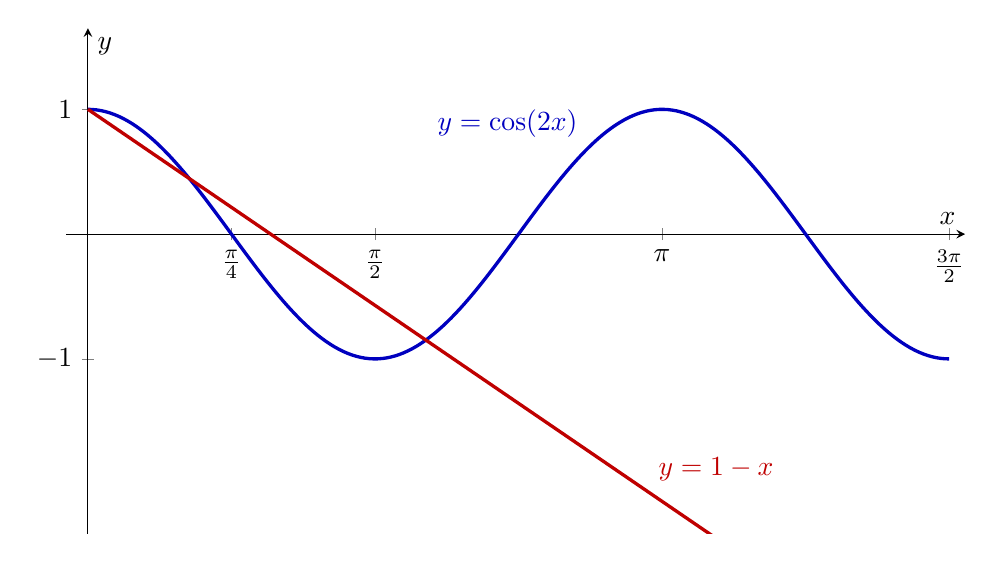
\begin{tikzpicture}
\pgfmathsetmacro{\xpi}{pi}
\pgfmathsetmacro{\xquarter}{pi/4}
\pgfmathsetmacro{\xhalf}{pi/2}
\pgfmathsetmacro{\xthreehalfpi}{3*pi/2}
\begin{axis}[
    width=13cm, height=8cm,
    axis lines=middle,
    xlabel={$x$}, ylabel={$y$},
    xmin=-0.12, xmax=4.8,
    ymin=-2.4, ymax=1.65,
    xtick={0,\xquarter,\xhalf,\xpi, \xthreehalfpi},
    xticklabels={$0$,$\frac{\pi}{4}$,$\frac{\pi}{2}$,$\pi$, $\frac{3\pi}{2}$},
    ytick={-1,1},
    yticklabels={$-1$,$1$},
    clip=true
]
\addplot[blue!75!black, very thick, domain=0:\xthreehalfpi, samples=200]
    {cos(deg(2*x))}
    node[pos=0.6, above left, blue!75!black] {$y=\cos(2x)$};
\addplot[red!75!black, very thick, domain=0:\xthreehalfpi, samples=2]
    {1-x}
    node[pos=0.65, above right, red!75!black] {$y=1-x$};
\end{axis}
\end{tikzpicture}
% end q000123 figure F1
\end{djsSolutionFigure}

Our sketch shows us three intersection points. 

Therefore there are three real solution to the original equation and the correct option is then \textbf{D}.
% end q000123 solution
\end{djsSolution}
\end{enumerate}
\clearpage
\thispagestyle{djssolutions}
\vspace*{8pt}
\djsTopicLine{Integration}
\begin{enumerate}[label=\textbf{\arabic*.},leftmargin=*,itemsep=0pt,start=4]
\questionitem[Integration]
% begin q000014 stem
Use the trapezium rule with $4$ equal strips to estimate \[ \int_{1}^{5} \ln x\,\,\mathrm{d}x \]
% end q000014 stem

\par\vspace*{12pt}
\begin{tabularx}{\linewidth}{@{}>{\bfseries}l Y@{}}
A &
% begin q000014 choice A
$\dfrac{1}{2}\ln(120)$
% end q000014 choice A
\\[0.8em]
B &
% begin q000014 choice B
$\dfrac{1}{2}\ln(180)$
% end q000014 choice B
\\[0.8em]
C &
% begin q000014 choice C
$\dfrac{1}{2}\ln(240)$
% end q000014 choice C
\\[0.8em]
D &
% begin q000014 choice D
$\dfrac{1}{2}\ln(720)$
% end q000014 choice D
\\[0.8em]
E &
% begin q000014 choice E
$\dfrac{1}{2}\ln(2880)$
% end q000014 choice E
\\[0.8em]
F &
% begin q000014 choice F
$\dfrac{1}{2}\ln(14400)$
% end q000014 choice F
\\
\end{tabularx}

\begin{djsSolution}{E}
% begin q000014 solution
For $n$ equal strips, the trapezium rule is
\[
\int_{x_0}^{x_n}y\,\mathrm{d}x\approx\frac{h}{2}\bigl[y_0+y_n+2(y_1+\cdots+y_{n-1})\bigr]
\]
Here $h$ is the width of each strip, and $y_i$ is the height of the curve at the $i$th division point. The end heights $y_0$ and $y_n$ are counted once; each height between them is shared by two trapezia and counted twice.

First, sketch the curve over the interval being estimated.

\begin{djsSolutionFigure}
% begin q000014 figure F1
\begin{tikzpicture}
\begin{axis}[
    width=12.5cm, height=6.4cm,
    xmin=0, xmax=5.6,
    ymin=-0.8, ymax=1.9,
    axis lines=middle,
    axis line style={black, thick, -},
    xlabel={$x$}, ylabel={$y$},
    xtick={1,2,3,4,5}, ytick=\empty,
    tick style={black},
    clip=true
]
\addplot[blue!70!black, very thick, domain=0.55:5.35, samples=180]
    {ln(x)} node[pos=0.86, above left] {$y=\ln x$};
\end{axis}
\end{tikzpicture}
% end q000014 figure F1
\end{djsSolutionFigure}

On the same curve, draw straight edges between the heights at $x=1,2,3,4,5$. These form the four strips used by the rule.

\begin{djsSolutionFigure}
% begin q000014 figure F2
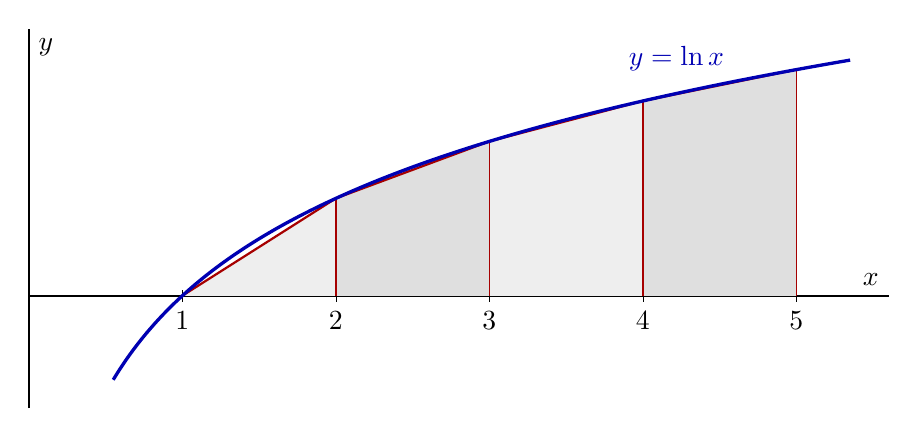
\begin{tikzpicture}
\pgfmathsetmacro{\htwo}{ln(2)}
\pgfmathsetmacro{\hthree}{ln(3)}
\pgfmathsetmacro{\hfour}{ln(4)}
\pgfmathsetmacro{\hfive}{ln(5)}
\begin{axis}[
    width=12.5cm, height=6.4cm,
    xmin=0, xmax=5.6,
    ymin=-0.8, ymax=1.9,
    axis lines=middle,
    axis line style={black, thick, -},
    xlabel={$x$}, ylabel={$y$},
    xtick={1,2,3,4,5}, ytick=\empty,
    tick style={black},
    clip=true
]
\fill[gray!13] (axis cs:1,0) -- (axis cs:2,0) -- (axis cs:2,\htwo) -- cycle;
\fill[gray!25] (axis cs:2,0) -- (axis cs:3,0) -- (axis cs:3,\hthree) -- (axis cs:2,\htwo) -- cycle;
\fill[gray!13] (axis cs:3,0) -- (axis cs:4,0) -- (axis cs:4,\hfour) -- (axis cs:3,\hthree) -- cycle;
\fill[gray!25] (axis cs:4,0) -- (axis cs:5,0) -- (axis cs:5,\hfive) -- (axis cs:4,\hfour) -- cycle;
\draw[red!65!black, thick] (axis cs:1,0) -- (axis cs:2,\htwo) -- (axis cs:3,\hthree) -- (axis cs:4,\hfour) -- (axis cs:5,\hfive);
\draw[red!65!black, semithick] (axis cs:2,0) -- (axis cs:2,\htwo);
\draw[red!65!black, semithick] (axis cs:3,0) -- (axis cs:3,\hthree);
\draw[red!65!black, semithick] (axis cs:4,0) -- (axis cs:4,\hfour);
\draw[red!65!black, semithick] (axis cs:5,0) -- (axis cs:5,\hfive);
\addplot[blue!70!black, very thick, domain=0.55:5.35, samples=180]
    {ln(x)} node[pos=0.86, above left] {$y=\ln x$};
\end{axis}
\end{tikzpicture}
% end q000014 figure F2
\end{djsSolutionFigure}

The strips have width
\[
h=\frac{5-1}{4}=1
\]
The five heights are
\[
\begin{aligned}
y_0&=\ln 1=0\\
y_1&=\ln 2\\
y_2&=\ln 3\\
y_3&=\ln 4\\
y_4&=\ln 5
\end{aligned}
\]
Substituting into the rule gives
\[
\int_1^5\ln x\,\mathrm{d}x\approx\frac12\bigl[0+\ln 5+2(\ln 2+\ln 3+\ln 4)\bigr]
\]
Use the logarithm laws one step at a time:
\[
\begin{aligned}
\int_1^5\ln x\,\mathrm{d}x
&\approx\frac12\bigl[\ln 5+2(\ln 6+\ln 4)\bigr]\\
&=\frac12\bigl[\ln 5+2\ln 24\bigr]\\
&=\frac12\bigl[\ln 5+\ln(24^2)\bigr]\\
&=\frac12\bigl[\ln 5+\ln 576\bigr]\\
&=\frac12\ln(5\times576)\\
&=\frac12\ln 2880
\end{aligned}
\]
The correct option is \textbf{E}.
% end q000014 solution
\end{djsSolution}
\end{enumerate}
\clearpage
\thispagestyle{djssolutions}
\vspace*{8pt}
\djsTopicLine{Coordinate Geometry}
\begin{enumerate}[label=\textbf{\arabic*.},leftmargin=*,itemsep=0pt,start=5]
\questionitem[Coordinate Geometry]
% begin q000661 stem
The points $A$ and $B$ have coordinates $(0,0)$ and $(10,0)$ respectively. 

A circle has diameter $AB$.

The point $C$ lies on the circle above the $x$-axis, with $AC=6$ and $BC=8$.

The tangent to the circle at $C$ meets the lines $x=0$ and $x=10$ at $P$ and $Q$ respectively.

What is the length $PQ$?
% end q000661 stem

\begin{center}
% begin q000661 diagram
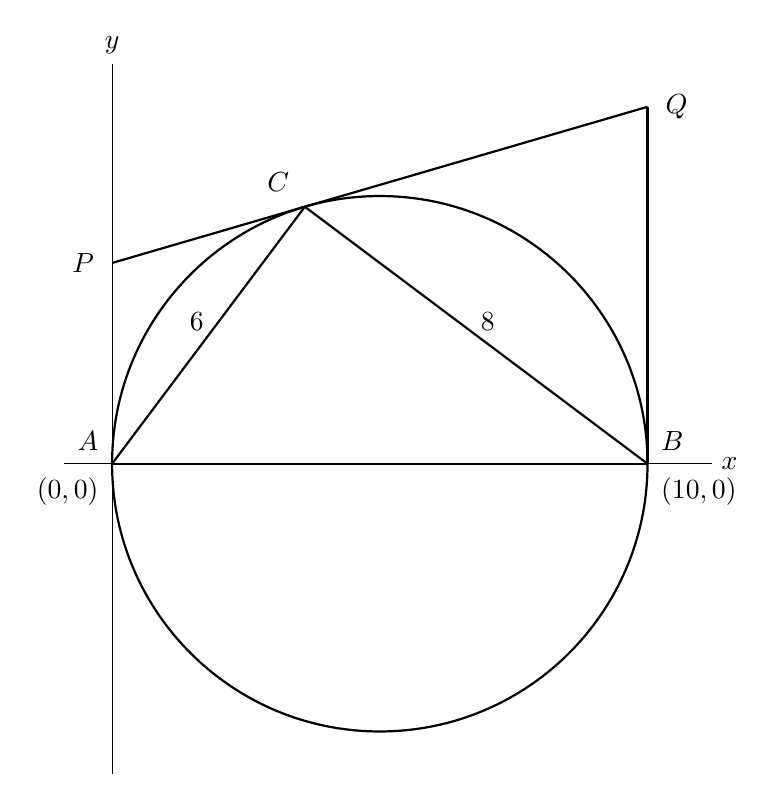
\begin{tikzpicture}[x=0.68cm,y=0.68cm]
\def\ABlen{10}
\pgfmathsetmacro{\rad}{\ABlen/2}
\pgfmathsetmacro{\Ox}{\ABlen/2}
\pgfmathsetmacro{\Cx}{18/5}
\pgfmathsetmacro{\Cy}{24/5}
\pgfmathsetmacro{\Py}{15/4}
\pgfmathsetmacro{\Qy}{20/3}
\pgfmathsetmacro{\xmin}{-0.9}
\pgfmathsetmacro{\xmax}{\ABlen+1.2}
\pgfmathsetmacro{\ymin}{-\rad-0.8}
\pgfmathsetmacro{\ymax}{\Qy+0.8}

\coordinate (A) at (0,0);
\coordinate (B) at (\ABlen,0);
\coordinate (O) at (\Ox,0);
\coordinate (C) at (\Cx,\Cy);
\coordinate (P) at (0,\Py);
\coordinate (Q) at (\ABlen,\Qy);

% Coordinate axes
\draw[black] (\xmin,0) -- (\xmax,0) node[right] {$x$};
\draw[black] (0,\ymin) -- (0,\ymax) node[above] {$y$};

% Circle and geometric segments
\draw[thick,black] (O) circle (\rad);
\draw[thick,black] (A) -- (B);
\draw[thick,black] (A) -- (C)
    node[midway,above left, yshift=-2pt, xshift=2pt] {$6$};
\draw[thick,black] (C) -- (B)
    node[midway,above right, yshift=-2pt, xshift=-2pt] {$8$};
\draw[thick,black] (P) -- (Q);
\draw[thick,black] (B) -- (Q);

% Point and coordinate labels
\node[above left=2pt] at (A) {$A$};
\node[below left=2pt] at (A) {$(0,0)$};
\node[above right=2pt] at (B) {$B$};
\node[below right=2pt] at (B) {$(10,0)$};
\node[above left=3pt] at (C) {$C$};
\node[left=3pt] at (P) {$P$};
\node[right=3pt] at (Q) {$Q$};
\end{tikzpicture}
% end q000661 diagram
\end{center}

\par\vspace*{12pt}
\begin{tabularx}{\linewidth}{@{}>{\bfseries}l Y@{}}
A &
% begin q000661 choice A
$\dfrac{35}{12}$
% end q000661 choice A
\\[0.8em]
B &
% begin q000661 choice B
$\dfrac{15}{4}$
% end q000661 choice B
\\[0.8em]
C &
% begin q000661 choice C
$\dfrac{20}{3}$
% end q000661 choice C
\\[0.8em]
D &
% begin q000661 choice D
$10$
% end q000661 choice D
\\[0.8em]
E &
% begin q000661 choice E
$\dfrac{125}{12}$
% end q000661 choice E
\\[0.8em]
F &
% begin q000661 choice F
$\dfrac{125}{6}$
% end q000661 choice F
\\
\end{tabularx}

\begin{djsSolution}{E}
% begin q000661 solution
Because $AB$ is a diameter, the angle in the semicircle is a right angle:
\[
\angle ACB=90^\circ
\]

Let $O$ be the centre of the circle, and let $D$ be the foot of the perpendicular from $C$ to $AB$. 

Write $\theta=\angle BAC$.

The following sketch shows the resulting geometry:

\begin{djsSolutionFigure}
% begin q000661 figure F1
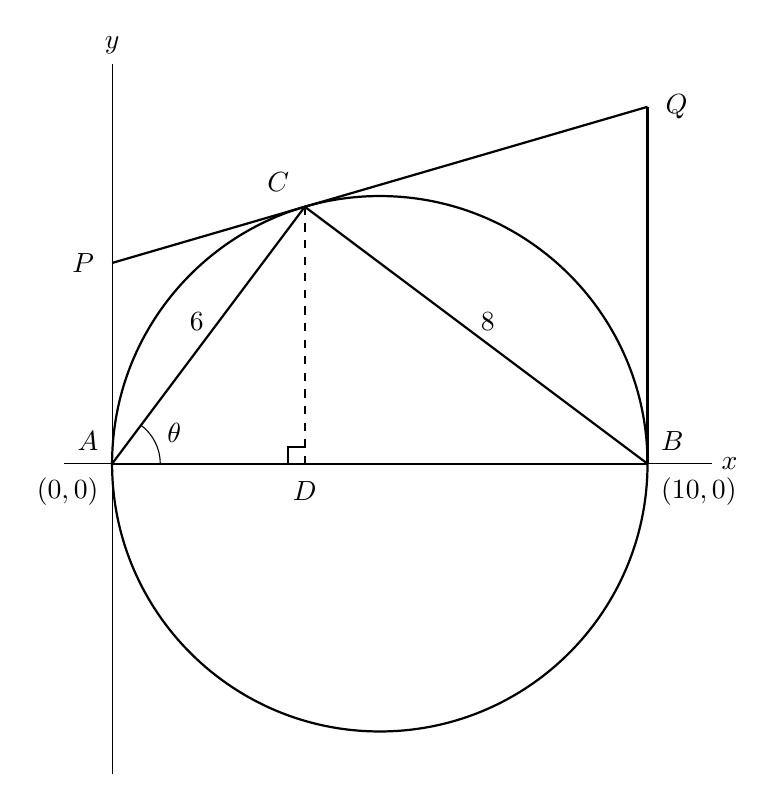
\begin{tikzpicture}[x=0.68cm,y=0.68cm]
\def\ABlen{10}
\pgfmathsetmacro{\rad}{\ABlen/2}
\pgfmathsetmacro{\Ox}{\ABlen/2}
\pgfmathsetmacro{\Cx}{18/5}
\pgfmathsetmacro{\Cy}{24/5}
\pgfmathsetmacro{\Py}{15/4}
\pgfmathsetmacro{\Qy}{20/3}
\pgfmathsetmacro{\thetaAngle}{atan2(\Cy,\Cx)}
\pgfmathsetmacro{\xmin}{-0.9}
\pgfmathsetmacro{\xmax}{\ABlen+1.2}
\pgfmathsetmacro{\ymin}{-\rad-0.8}
\pgfmathsetmacro{\ymax}{\Qy+0.8}

\coordinate (A) at (0,0);
\coordinate (B) at (\ABlen,0);
\coordinate (O) at (\Ox,0);
\coordinate (C) at (\Cx,\Cy);
\coordinate (D) at (\Cx,0);
\coordinate (P) at (0,\Py);
\coordinate (Q) at (\ABlen,\Qy);

% Coordinate axes
\draw[black] (\xmin,0) -- (\xmax,0) node[right] {$x$};
\draw[black] (0,\ymin) -- (0,\ymax) node[above] {$y$};

% Circle and geometric segments
\draw[thick,black] (O) circle (\rad);
\draw[thick,black] (A) -- (B);
\draw[thick,black] (A) -- (C)
    node[midway,above left, yshift=-2pt, xshift=2pt] {$6$};
\draw[thick,black] (C) -- (B)
    node[midway,above right, yshift=-2pt, xshift=-2pt] {$8$};
\draw[thick,black] (P) -- (Q);
\draw[thick,black] (B) -- (Q);

% Perpendicular from C to AB and angle at A
\draw[thick,dashed,black] (C) -- (D);
\draw[thick,black]
    ($(D)+(-0.32,0)$) -- ($(D)+(-0.32,0.32)$) -- ($(D)+(0,0.32)$);
\draw[black] (0.9,0) arc[start angle=0,end angle=\thetaAngle,radius=0.9];
\node at ({1.3*cos(\thetaAngle/2)},{1.3*sin(\thetaAngle/2)}) {$\theta$};

% Point and coordinate labels
\node[above left=2pt] at (A) {$A$};
\node[below left=2pt] at (A) {$(0,0)$};
\node[above right=2pt] at (B) {$B$};
\node[below right=2pt] at (B) {$(10,0)$};
\node[above left=3pt] at (C) {$C$};
\node[below=3pt] at (D) {$D$};
\node[left=3pt] at (P) {$P$};
\node[right=3pt] at (Q) {$Q$};
\end{tikzpicture}
% end q000661 figure F1
\end{djsSolutionFigure}

In right-angled triangle $BAC$, $AB=10$, so
\[
\sin\theta=\frac{BC}{AB}=\frac{8}{10}=\frac45
\]

Similarly,
\[
\cos\theta=\frac{AC}{AB}=\frac{6}{10}=\frac35
\]

Now use right-angled triangle $ACD$. Its horizontal side is
\[
AD=AC\cos\theta=6\left(\frac35\right)=\frac{18}{5}
\]

Its vertical side is
\[
CD=AC\sin\theta=6\left(\frac45\right)=\frac{24}{5}
\]

Since $A=(0,0)$ and $C$ is above the $x$-axis, these are the coordinates of $C$:
\[
C=\left(\frac{18}{5},\frac{24}{5}\right)
\]

The centre is the midpoint of $AB$, so
\[
O=(5,0)
\]

Hence the gradient of the radius $OC$ is
\[
\begin{aligned}
\text{gradient of }OC
&=\frac{\frac{24}{5}-0}{\frac{18}{5}-5}\\[8pt]
&=\frac{\frac{24}{5}}{-\frac75}\\[8pt]
&=-\frac{24}{7}
\end{aligned}
\]

The tangent $PQ$ is perpendicular to $OC$, so its gradient is the negative reciprocal:
\[
\text{gradient of }PQ=-\frac{1}{-\frac{24}{7}}=\frac{7}{24}
\]

Draw a horizontal line from $P$ to meet the vertical line $BQ$ at $R$. The horizontal distance from $x=0$ to $x=10$ is $10$, so
\[
PR=10
\]

The gradient of $PQ$ is its vertical rise divided by its horizontal run. Thus
\[
\frac{RQ}{PR}=\frac{7}{24}
\]

Substituting $PR=10$ gives
\[
\frac{RQ}{10}=\frac{7}{24}
\]

Therefore
\[
RQ=\frac{70}{24}
\]

Simplifying,
\[
RQ=\frac{35}{12}
\]

\begin{djsSolutionFigure}
% begin q000661 figure F2
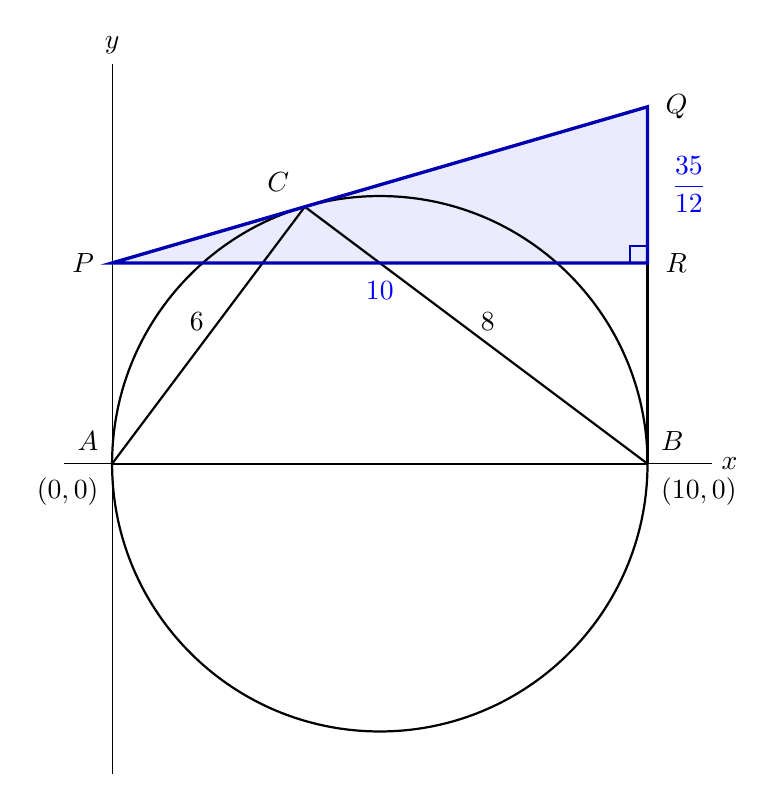
\begin{tikzpicture}[x=0.68cm,y=0.68cm]
\def\ABlen{10}
\pgfmathsetmacro{\rad}{\ABlen/2}
\pgfmathsetmacro{\Ox}{\ABlen/2}
\pgfmathsetmacro{\Cx}{18/5}
\pgfmathsetmacro{\Cy}{24/5}
\pgfmathsetmacro{\Py}{15/4}
\pgfmathsetmacro{\Qy}{20/3}
\pgfmathsetmacro{\xmin}{-0.9}
\pgfmathsetmacro{\xmax}{\ABlen+1.2}
\pgfmathsetmacro{\ymin}{-\rad-0.8}
\pgfmathsetmacro{\ymax}{\Qy+0.8}

\coordinate (A) at (0,0);
\coordinate (B) at (\ABlen,0);
\coordinate (O) at (\Ox,0);
\coordinate (C) at (\Cx,\Cy);
\coordinate (P) at (0,\Py);
\coordinate (Q) at (\ABlen,\Qy);
\coordinate (R) at (\ABlen,\Py);
\fill[blue!8] (P) -- (R) -- (Q) -- cycle;

% Coordinate axes
\draw[black] (\xmin,0) -- (\xmax,0) node[right] {$x$};
\draw[black] (0,\ymin) -- (0,\ymax) node[above] {$y$};

% Circle and geometric segments
\draw[thick,black] (O) circle (\rad);
\draw[thick,black] (A) -- (B);
\draw[thick,black] (A) -- (C)
    node[midway,above left, yshift=-2pt, xshift=2pt] {$6$};
\draw[thick,black] (C) -- (B)
    node[midway,above right, yshift=-2pt, xshift=-2pt] {$8$};
\draw[thick,black] (P) -- (Q);
\draw[thick,black] (B) -- (Q);

% Added right triangle
\draw[very thick,blue!70!black] (P) -- (R) -- (Q) -- cycle;
\draw[blue!70!black,thick]
    ($(R)+(-0.32,0)$) -- ($(R)+(-0.32,0.32)$) -- ($(R)+(0,0.32)$);

% Point and coordinate labels
\node[above left=2pt] at (A) {$A$};
\node[below left=2pt] at (A) {$(0,0)$};
\node[above right=2pt] at (B) {$B$};
\node[below right=2pt] at (B) {$(10,0)$};
\node[above left=3pt] at (C) {$C$};
\node[left=3pt] at (P) {$P$};
\node[right=3pt] at (Q) {$Q$};
\node[right=3pt] at (R) {$R$};
\path (P) -- (R) node[midway,below=3pt, blue, thick] {$10$};
\path (R) -- (Q) node[midway,right=5pt, blue, thick] {$\dfrac{35}{12}$};
\end{tikzpicture}
% end q000661 figure F2
\end{djsSolutionFigure}

Triangle $PRQ$ is right-angled at $R$. By Pythagoras,
\[
PQ=\sqrt{PR^2+RQ^2}
\]

Substituting the two lengths,
\[
PQ=\sqrt{10^2+\left(\frac{35}{12}\right)^2}
\]

To simplify by hand, write both lengths as multiples of $\frac{5}{12}$:
\[
PQ=\sqrt{\left(\frac{5}{12}\times24\right)^2
+\left(\frac{5}{12}\times7\right)^2}
\]

Factor out the common square before evaluating the remaining squares:
\[
\begin{aligned}
PQ&=\sqrt{\left(\frac{5}{12}\right)^2(24^2+7^2)}\\
&=\frac{5}{12}\sqrt{24^2+7^2}\\
&=\frac{5}{12}\sqrt{576+49}\\
&=\frac{5}{12}\sqrt{625}\\
&=\frac{5\times25}{12}
\end{aligned}
\]

Therefore
\[
PQ=\frac{125}{12}
\]

The correct option is \textbf{E}.
% end q000661 solution
\end{djsSolution}
\end{enumerate}
\clearpage
\thispagestyle{djssolutions}
\vspace*{8pt}
\djsTopicLine{Integration}
\begin{enumerate}[label=\textbf{\arabic*.},leftmargin=*,itemsep=0pt,start=6]
\questionitem[Integration]
% begin q000611 stem
Let $k$ be a positive real constant. The function $f(x)$ is defined for $x > 0$ by

\[ f(x) = \int_1^x \frac{t - k}{\sqrt{t}} \, \mathrm{d}t \]

What is the complete set of values of $k$ for which the equation $f(x) = 0$ has exactly two distinct real solutions for $x > 0$?
% end q000611 stem

\par\vspace*{12pt}
\begin{tabularx}{\linewidth}{@{}>{\bfseries}l Y@{}}
A &
% begin q000611 choice A
$k > 1$
% end q000611 choice A
\\[0.8em]
B &
% begin q000611 choice B
$k > \frac{1}{3}$
% end q000611 choice B
\\[0.8em]
C &
% begin q000611 choice C
$k > \frac{1}{3}$ and $k \neq 1$
% end q000611 choice C
\\[0.8em]
D &
% begin q000611 choice D
$\frac{1}{3} < k < 1$
% end q000611 choice D
\\[0.8em]
E &
% begin q000611 choice E
$k > 0$ and $k \neq 1$
% end q000611 choice E
\\[0.8em]
F &
% begin q000611 choice F
$k \ge \frac{1}{4}$ and $k \neq 1$
% end q000611 choice F
\\
\end{tabularx}

\begin{djsSolution}{C}
% begin q000611 solution
First evaluate the integral:
\[
\begin{aligned}
f(x)
&=\int_1^x\left(t^{1/2}-kt^{-1/2}\right)\,\mathrm{d}t\\[8pt]
&=\left[\frac{2}{3}t^{3/2}-2kt^\frac{1}{2}\right] _1^x\\[8pt]
&=\frac{2}{3}(x^{3/2}-1)-2k(\sqrt x-1)
\end{aligned}
\]

Set $y=\sqrt x$. Since $x>0$, we require $y>0$, and each positive value of $y$ corresponds to exactly one value of $x$. The equation $f(x)=0$ becomes
\[
y^3-3ky+3k-1=0
\]

We already know that $x=1$ is a solution, because the integral from $1$ to $1$ is zero. Thus $y=1$ is a root of this cubic, so $y-1$ is a factor.

Dividing the cubic by $y-1$ gives
\[
(y-1)(y^2+y+1-3k)=0
\]

The root $y=1$ is always present. To obtain exactly two distinct positive roots overall, the quadratic must have either one positive root different from $1$, or two distinct positive roots, one of which is $1$.

Using the quadratic formula, the roots of
\[
y^2+y+1-3k=0
\]
are
\[
y=\frac{-1\pm\sqrt{1-4(1-3k)}}{2}
=\frac{-1\pm\sqrt{12k-3}}{2}
\]

When these roots are real, the root
\[
\frac{-1-\sqrt{12k-3}}{2}
\]
is always negative. Thus the quadratic cannot have two positive roots. We need its other root to be positive and different from $1$.

For this root to be positive,
\[
\frac{-1+\sqrt{12k-3}}{2}>0
\]
Hence
\[
\sqrt{12k-3}>1
\]
Squaring and rearranging gives
\[
12k-3>1
\quad\Longrightarrow\quad
k>\frac13
\]
We must also exclude the case where this root equals $1$:
\[
\frac{-1+\sqrt{12k-3}}{2}=1
\quad\Longrightarrow\quad
\sqrt{12k-3}=3
\quad\Longrightarrow\quad
k=1
\]
Therefore the equation has exactly two distinct solutions for $x>0$ precisely when
\[
k>\frac13\quad\text{and}\quad k\ne1
\]
The correct option is \textbf{C}.

As a shortcut, the quadratic equation can be written as
\[
y^2+y=3k-1
\]
For $y>0$, the left-hand side increases from $0$ without bound, so there is exactly one positive root precisely when $k>\frac13$. Substituting $y=1$ then identifies $k=1$ as the value to exclude.\\[5pt]

\textit{Alternative Solution:} (Graph Sketching)

The Fundamental Theorem of Calculus, which is on the TMUA specification, tells us that differentiating an integral with respect to its upper limit gives the integrand evaluated at that limit:
\[
\frac{\mathrm{d}}{\mathrm{d}x}\left(\int_a^x g(t)\,\mathrm{d}t\right)=g(x)
\]

Applying this here gives
\[
f'(x)=\frac{x-k}{\sqrt x}
\]

Since $\sqrt x>0$, the graph decreases for $0<x<k$ and increases for $x>k$. It therefore has a minimum at $x=k$, and can cross the axis at most once on each side of this minimum.

We also know that
\[
f(1)=\int_1^1\frac{t-k}{\sqrt t}\,\mathrm{d}t=0
\]

To determine whether there is another zero, we need to know how the graph behaves near $x=0$ and for large positive $x$. Evaluating the integral gives
\[
f(x)=\frac23(x^{3/2}-1)-2k(\sqrt x-1)
\]

As $x$ approaches $0$ from above, both $x^{3/2}$ and $\sqrt x$ approach $0$, so $f(x)$ approaches
\[
2k-\frac23
\]

For large positive $x$, the $x^{3/2}$ term dominates the $\sqrt x$ term, so $f(x)$ increases without bound.

First suppose $0<k<1$. The minimum lies to the left of $x=1$ and is below the axis, since the graph increases from that minimum to $f(1)=0$. There is a second crossing before the minimum precisely when the graph starts above the axis near $x=0$:
\[
2k-\frac23>0
\]
Thus, within this case, there are two distinct solutions precisely when
\[
\frac13<k<1
\]
If $k=\frac13$, the graph approaches height $0$ as $x$ approaches $0$, but $x=0$ is excluded. The graph decreases below the axis before reaching its minimum, so there is no additional solution.

If $0<k<\frac13$, the graph is already below the axis near $x=0$ and decreases further before reaching its minimum. Again, there is no additional solution.

If $k=1$, the minimum occurs at $x=1$ and has value $0$. The graph touches the axis there, giving only one solution.

If $k>1$, the graph decreases from $f(1)=0$ to a negative minimum at $x=k$. It then increases without bound, so it crosses the axis exactly once more after $x=k$.

The sketches below summarise these five cases. The first two have just one crossing, while the third has two. When $k=1$, the graph only touches the axis; when $k>1$, it crosses twice. Each open circle marks the height approached at $x=0$, which is excluded from the domain.

\begin{djsSolutionFigure}
% begin q000611 figure F1
\begin{tikzpicture}
% 0<k<1/3
\begin{scope}[shift={(0cm,0cm)},x=2.1cm,y=3.2cm]
  \draw[black!65,-{Stealth[length=2mm]}] (-0.10,0) -- (1.95,0) node[right] {$x$};
  \draw[black!65,-{Stealth[length=2mm]}] (0,-0.41) -- (0,0.91) node[above] {$f(x)$};
  \draw[black!65] (1/4,0) ++(0,-2pt) -- ++(0,4pt);
  \draw[black!65] (1,0) ++(0,-2pt) -- ++(0,4pt);
  \node[below=3pt] at (1/4,0) {$k$};
  \node[below=3pt] at (1,0) {$1$};
  \draw[blue!70!black,line width=1.05pt]
    plot[domain=0.001:1.8,samples=180]
    (\x,{2/3*(\x^(3/2)-1)-2*(1/4)*(sqrt(\x)-1)});
  \node[draw=black,fill=white,thick,circle,minimum size=5pt,inner sep=0pt]
    at (0,{2*(1/4)-2/3}) {};
  \node[anchor=south,yshift=4cm] at (0.9,0) {$0<k<\frac13$};
\end{scope}
% k=1/3
\begin{scope}[shift={(4.65cm,0cm)},x=2.1cm,y=3.2cm]
  \draw[black!65,-{Stealth[length=2mm]}] (-0.10,0) -- (1.95,0) node[right] {$x$};
  \draw[black!65,-{Stealth[length=2mm]}] (0,-0.34) -- (0,0.91) node[above] {$f(x)$};
  \draw[black!65] (1/3,0) ++(0,-2pt) -- ++(0,4pt);
  \draw[black!65] (1,0) ++(0,-2pt) -- ++(0,4pt);
  \node[below=3pt] at (1/3,0) {$k$};
  \node[below=3pt] at (1,0) {$1$};
  \draw[blue!70!black,line width=1.05pt]
    plot[domain=0.001:1.8,samples=180]
    (\x,{2/3*(\x^(3/2)-1)-2*(1/3)*(sqrt(\x)-1)});
  \node[draw=black,fill=white,thick,circle,minimum size=5pt,inner sep=0pt]
    at (0,0) {};
  \node[anchor=south,yshift=4cm] at (0.9,0) {$k=\frac13$};
\end{scope}
% 1/3<k<1
\begin{scope}[shift={(9.3cm,0cm)},x=2.1cm,y=5cm]
  \draw[black!65,-{Stealth[length=2mm]}] (-0.10,0) -- (1.95,0) node[right] {$x$};
  \draw[black!65,-{Stealth[length=2mm]}] (0,-0.10) -- (0,0.74) node[above] {$f(x)$};
  \draw[black!65] (2/3,0) ++(0,-2pt) -- ++(0,4pt);
  \draw[black!65] (1,0) ++(0,-2pt) -- ++(0,4pt);
  \node[above=3pt] at (2/3,0) {$k$};
  \node[below=3pt] at (1,0) {$1$};
  \draw[blue!70!black,line width=1.05pt]
    plot[domain=0.001:1.8,samples=180]
    (\x,{2/3*(\x^(3/2)-1)-2*(2/3)*(sqrt(\x)-1)});
  \node[draw=black,fill=white,thick,circle,minimum size=5pt,inner sep=0pt]
    at (0,{2*(2/3)-2/3}) {};
  \node[anchor=south,yshift=4cm] at (0.9,0) {$\frac13<k<1$};
\end{scope}
% k=1
\begin{scope}[shift={(2.25cm,-6.75cm)},x=2.1cm,y=2.6cm]
  \draw[black!65,-{Stealth[length=2mm]}] (-0.10,0) -- (1.95,0) node[right] {$x$};
  \draw[black!65,-{Stealth[length=2mm]}] (0,-0.16) -- (0,1.48) node[above] {$f(x)$};
  \draw[black!65] (1,0) ++(0,-2pt) -- ++(0,4pt);
  \node[below=3pt] at (1,0) {$k=1$};
  \draw[blue!70!black,line width=1.05pt]
    plot[domain=0.001:1.8,samples=180]
    (\x,{2/3*(\x^(3/2)-1)-2*(sqrt(\x)-1)});
  \node[draw=black,fill=white,thick,circle,minimum size=5pt,inner sep=0pt]
    at (0,{2-2/3}) {};
  \node[anchor=south,yshift=4.3cm] at (0.9,0) {$k=1$};
\end{scope}
% k>1
\begin{scope}[shift={(7.05cm,-6.75cm)},x=1.67cm,y=1.8cm]
  \draw[black!65,-{Stealth[length=2mm]}] (-0.12,0) -- (2.78,0) node[right] {$x$};
  \draw[black!65,-{Stealth[length=2mm]}] (0,-0.25) -- (0,2.55) node[above] {$f(x)$};
  \draw[black!65] (1,0) ++(0,-2pt) -- ++(0,4pt);
  \draw[black!65] (3/2,0) ++(0,-2pt) -- ++(0,4pt);
  \node[above=3pt] at (1,0) {$1$};
  \node[above=3pt] at (3/2,0) {$k$};
  \draw[blue!70!black,line width=1.05pt]
    plot[domain=0.001:2.65,samples=220]
    (\x,{2/3*(\x^(3/2)-1)-2*(3/2)*(sqrt(\x)-1)});
  \node[draw=black,fill=white,thick,circle,minimum size=5pt,inner sep=0pt]
    at (0,{2*(3/2)-2/3}) {};
  \node[anchor=south,yshift=5cm] at (1.35,0) {$k>1$};
\end{scope}
\end{tikzpicture}
% end q000611 figure F1
\end{djsSolutionFigure}

Combining the two cases with exactly two distinct solutions gives
\[
\frac13<k<1\quad\text{or}\quad k>1
\]

Equivalently,
\[
k>\frac13\quad\text{and}\quad k\ne1
\]

The correct option is \textbf{C}.
% end q000611 solution
\end{djsSolution}
\end{enumerate}
\clearpage
\thispagestyle{djssolutions}
\vspace*{8pt}
\djsTopicLine{Geometry}
\begin{enumerate}[label=\textbf{\arabic*.},leftmargin=*,itemsep=0pt,start=7]
\questionitem[Geometry]
% begin q000652 stem
A straight line $\ell$ is drawn, and three circles lie on the same side of $\ell$. Each circle touches $\ell$ at exactly one point.

Circle $A$ has radius $1$ and circle $B$ has radius $4$, and these two circles touch each other.

Circle $C$ lies in the space between circle $A$, circle $B$ and the line $\ell$, touching circle $A$, circle $B$ and $\ell$.

What is the radius of circle $C$?
% end q000652 stem

\begin{center}
% begin q000652 diagram
\begin{tikzpicture}[scale=0.9]
\def\rA{1}
\def\rB{4}
\def\rC{4/9}

\coordinate (Acenter) at (0,\rA);
\coordinate (Bcenter) at (4,\rB);
\coordinate (Ccenter) at (4/3,\rC);
\coordinate (Ctip) at ($(Ccenter)+(300:\rC)$);
\coordinate (CLabelPos) at ($(Ccenter)+(0.72,-1.03)$);

\draw[thick, black] ({-\rA-0.45},0) -- ({4+\rB+0.45},0)
    node[right] {$\ell$};
\draw[thick, black] (Acenter) circle (\rA);
\draw[thick, black] (Bcenter) circle (\rB);
\draw[thick, black] (Ccenter) circle (\rC);

\node at (Acenter) {$A$};
\node at (Bcenter) {$B$};
\node (CLabel) at (CLabelPos) {$C$};
\draw[black] (CLabel.north west) -- (Ctip);
\end{tikzpicture}
% end q000652 diagram
\end{center}

\par\vspace*{12pt}
\begin{tabularx}{\linewidth}{@{}>{\bfseries}l Y@{}}
A &
% begin q000652 choice A
$\dfrac{2}{9}$
% end q000652 choice A
\\[0.8em]
B &
% begin q000652 choice B
$\dfrac{4}{9}$
% end q000652 choice B
\\[0.8em]
C &
% begin q000652 choice C
$\dfrac{1}{2}$
% end q000652 choice C
\\[0.8em]
D &
% begin q000652 choice D
$\dfrac{16}{25}$
% end q000652 choice D
\\[0.8em]
E &
% begin q000652 choice E
$\dfrac{2}{3}$
% end q000652 choice E
\\[0.8em]
F &
% begin q000652 choice F
$\dfrac{4}{5}$
% end q000652 choice F
\\[0.8em]
G &
% begin q000652 choice G
$\dfrac{8}{9}$
% end q000652 choice G
\\
\end{tabularx}

\begin{djsSolution}{B}
% begin q000652 solution
Let $r$ be the radius of circle $C$. For two circles that touch externally, the distance between their centres is the sum of their radii. 

Because each circle touches $\ell$, its centre is one radius above the line.

First consider circles $A$ and $B$. Their centres are $1+4=5$ apart, and the difference in their heights is $4-1=3$. 

These are the hypotenuse and vertical side of the right-angled triangle shown below.

\begin{djsSolutionFigure}
% begin q000652 figure F1
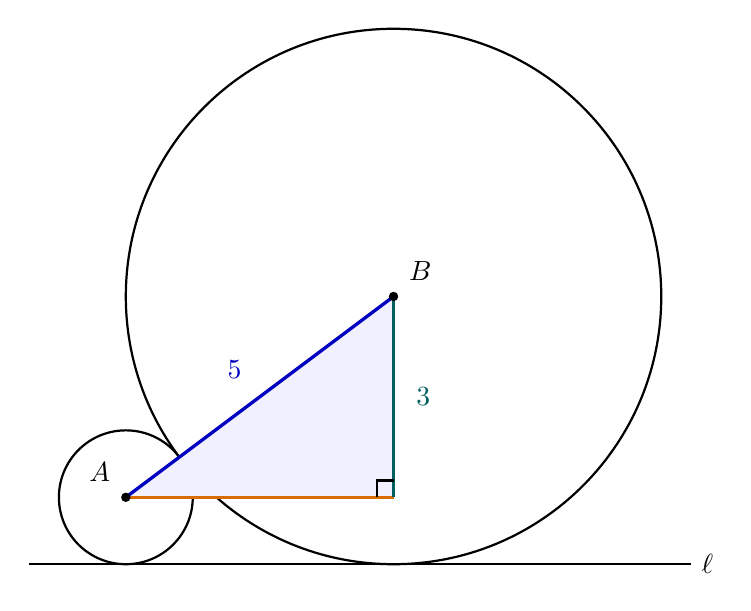
\begin{tikzpicture}[scale=0.85]
\coordinate (Acenter) at (0,1);
\coordinate (Bcenter) at (4,4);
\coordinate (ABfoot) at (4,1);

% Line and the two relevant circles
\draw[thick,black] (-1.45,0) -- (8.45,0) node[right] {$\ell$};
\draw[thick,black] (Acenter) circle (1);
\draw[thick,black] (Bcenter) circle (4);

% Right-angled triangle joining the centres
\fill[blue!6] (Acenter) -- (ABfoot) -- (Bcenter) -- cycle;
\draw[very thick,blue!75!black] (Acenter) -- (Bcenter)
    node[midway,above left=2mm,fill=white,inner sep=2pt] {$5$};
\draw[very thick,orange!85!black] (Acenter) -- (ABfoot);
\draw[very thick,teal!75!black] (ABfoot) -- (Bcenter)
    node[midway,right=2mm,fill=white,inner sep=2pt] {$3$};
\draw[thick,black] ($(ABfoot)+(-0.25,0)$)
    -- ($(ABfoot)+(-0.25,0.25)$)
    -- ($(ABfoot)+(0,0.25)$);

% Centres and labels
\fill (Acenter) circle (2pt);
\fill (Bcenter) circle (2pt);
\node[above left=3pt] at (Acenter) {$A$};
\node[above right=3pt] at (Bcenter) {$B$};
\end{tikzpicture}
% end q000652 figure F1
\end{djsSolutionFigure}

By Pythagoras, the horizontal side has length
\[
\sqrt{5^2-3^2}=\sqrt{25-9}=\sqrt{16}=4
\]

Now consider circles $A$ and $C$. Their centres are $1+r$ apart. 

Circle $C$ is the smaller circle in the gap, so $r<1$ and the difference in the heights of their centres is $1-r$. 

The next sketch shows the corresponding right-angled triangle, with circle $B$ omitted.

\begin{djsSolutionFigure}
% begin q000652 figure F2
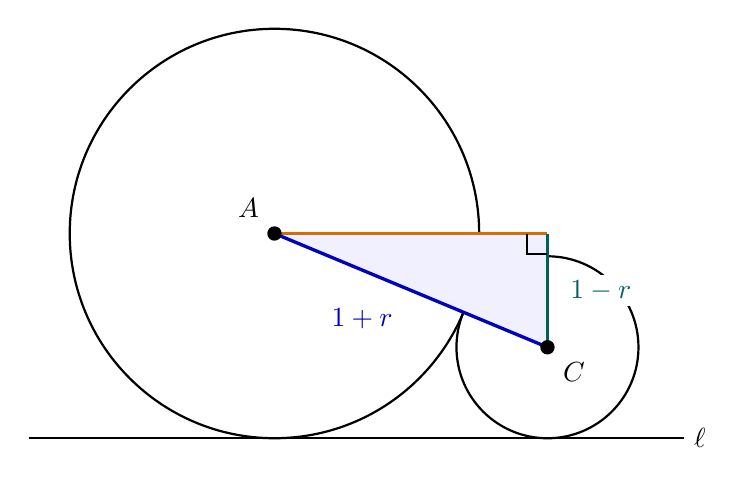
\begin{tikzpicture}[scale=2.6]
\def\rC{4/9}
\coordinate (Acenter) at (0,1);
\coordinate (Ccenter) at (4/3,\rC);
\coordinate (ACfoot) at (4/3,1);

% Line and the two relevant circles
\draw[thick,black] (-1.2,0) -- (2,0) node[right] {$\ell$};
\draw[thick,black] (Acenter) circle (1);
\draw[thick,black] (Ccenter) circle (\rC);

% Right-angled triangle joining the centres
\fill[blue!6] (Acenter) -- (ACfoot) -- (Ccenter) -- cycle;
\draw[very thick,blue!75!black] (Acenter) -- (Ccenter)
    node[midway,below left=2mm,fill=white,inner sep=2pt] {$1+r$};
\draw[very thick,orange!85!black] (Acenter) -- (ACfoot);
\draw[very thick,teal!75!black] (ACfoot) -- (Ccenter)
    node[midway,right=2mm,fill=white,inner sep=2pt] {$1-r$};
\draw[thick,black] ($(ACfoot)+(-0.10,0)$)
    -- ($(ACfoot)+(-0.10,-0.10)$)
    -- ($(ACfoot)+(0,-0.10)$);

% Centres and labels
\fill (Acenter) circle (1pt);
\fill (Ccenter) circle (1pt);
\node[above left=3pt] at (Acenter) {$A$};
\node[below right=3pt] at (Ccenter) {$C$};
\end{tikzpicture}
% end q000652 figure F2
\end{djsSolutionFigure}

By Pythagoras, its horizontal side has length
\[
\begin{aligned}
\sqrt{(1+r)^2-(1-r)^2}
&=\sqrt{(1+2r+r^2)-(1-2r+r^2)}\\[8pt]
&=\sqrt{4r}\\[8pt]
&=2\sqrt r
\end{aligned}
\]

Finally, consider circles $B$ and $C$. 

Their centres are $4+r$ apart, and the difference in their heights is $4-r$.

This gives the third right-angled triangle, shown below with circle $A$ omitted.

\begin{djsSolutionFigure}
% begin q000652 figure F3
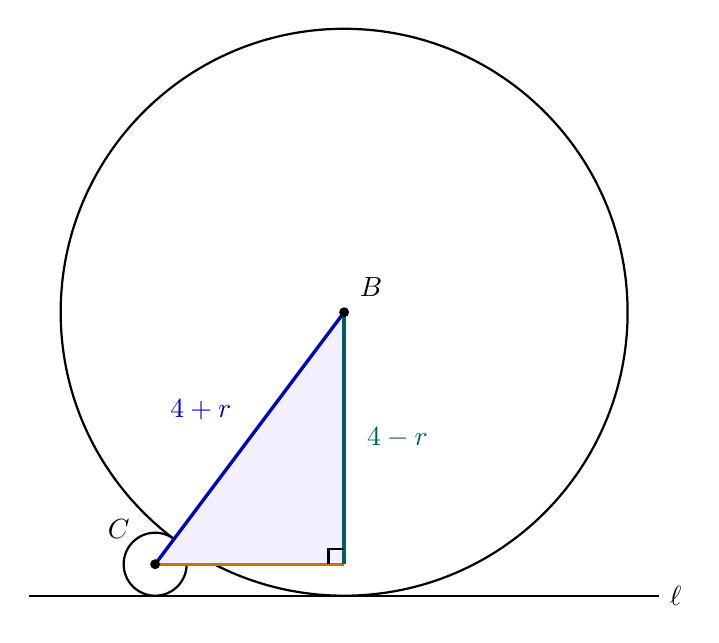
\begin{tikzpicture}[scale=0.9]
\def\rC{4/9}
\coordinate (Bcenter) at (4,4);
\coordinate (Ccenter) at (4/3,\rC);
\coordinate (BCfoot) at (4,\rC);

% Line and the two relevant circles
\draw[thick,black] (-0.45,0) -- (8.45,0) node[right] {$\ell$};
\draw[thick,black] (Bcenter) circle (4);
\draw[thick,black] (Ccenter) circle (\rC);

% Right-angled triangle joining the centres
\fill[blue!6] (Ccenter) -- (BCfoot) -- (Bcenter) -- cycle;
\draw[very thick,blue!75!black] (Ccenter) -- (Bcenter)
    node[midway,above left=2mm,fill=white,inner sep=2pt] {$4+r$};
\draw[very thick,orange!85!black] (Ccenter) -- (BCfoot);
\draw[very thick,teal!75!black] (BCfoot) -- (Bcenter)
    node[midway,right=2mm,fill=white,inner sep=2pt] {$4-r$};
\draw[thick,black] ($(BCfoot)+(-0.22,0)$)
    -- ($(BCfoot)+(-0.22,0.22)$)
    -- ($(BCfoot)+(0,0.22)$);

% Centres and labels
\fill (Bcenter) circle (2pt);
\fill (Ccenter) circle (2pt);
\node[above right=3pt] at (Bcenter) {$B$};
\node[above left=8pt] at (Ccenter) {$C$};
\end{tikzpicture}
% end q000652 figure F3
\end{djsSolutionFigure}

By Pythagoras, its horizontal side has length
\[
\begin{aligned}
\sqrt{(4+r)^2-(4-r)^2}
&=\sqrt{(16+8r+r^2)-(16-8r+r^2)}\\[8pt]
&=\sqrt{16r}\\[8pt]
&=4\sqrt r
\end{aligned}
\]

Since the centre of $C$ lies horizontally between the centres of $A$ and $B$, the two shorter horizontal lengths add to $4$:
\[
2\sqrt r+4\sqrt r=4
\]

Collecting terms,
\[
6\sqrt r=4
\]

Dividing by $6$,
\[
\sqrt r=\frac23
\]

Squaring,
\[
r=\left(\frac23\right)^2=\frac49
\]

The correct option is \textbf{B}.
% end q000652 solution
\end{djsSolution}
\end{enumerate}
\clearpage
\thispagestyle{djssolutions}
\vspace*{8pt}
\djsTopicLine{Probability \& Counting}
\begin{enumerate}[label=\textbf{\arabic*.},leftmargin=*,itemsep=0pt,start=8]
\questionitem[Probability \& Counting]
% begin q000562 stem
$N=2^7 \times 3^5$

One of the positive factors of $N$ that is divisible by $12$ is selected at random, with each such factor equally likely to be selected.

What is the probability that $N$ divided by the selected factor is a perfect square?
% end q000562 stem

\par\vspace*{12pt}
\begin{tabularx}{\linewidth}{@{}>{\bfseries}l Y@{}}
A &
% begin q000562 choice A
$\dfrac{1}{6}$
% end q000562 choice A
\\[0.8em]
B &
% begin q000562 choice B
$\dfrac{1}{5}$
% end q000562 choice B
\\[0.8em]
C &
% begin q000562 choice C
$\dfrac{1}{4}$
% end q000562 choice C
\\[0.8em]
D &
% begin q000562 choice D
$\dfrac{3}{10}$
% end q000562 choice D
\\[0.8em]
E &
% begin q000562 choice E
$\dfrac{1}{3}$
% end q000562 choice E
\\[0.8em]
F &
% begin q000562 choice F
$\dfrac{2}{5}$
% end q000562 choice F
\\
\end{tabularx}

\begin{djsSolution}{D}
% begin q000562 solution
Since $12=2^2\times3$, a selected factor must contain at least two powers of $2$ and one power of $3$. Write it as
\[
d=2^{2+i}3^{1+j}
\]
where the exponents cannot exceed those in $N$, so
\[
0\leq i\leq5,\qquad 0\leq j\leq4
\]
There are $6$ choices for $i$ and $5$ for $j$, giving
\[
6\times5=30
\]
equally likely factors.

For any such factor,
\[
\frac{N}{d}=\frac{2^7 3^5}{2^{2+i}3^{1+j}}
\]
Cancelling the powers gives
\[
\frac{N}{d}=2^{5-i}3^{4-j}
\]
A positive integer is a perfect square if every exponent in its prime factorisation is even, including an exponent of zero. Thus $5-i$ must be even, giving
\[
i=1,\ 3\text{ or }5
\]
Also, $4-j$ must be even, giving
\[
j=0,\ 2\text{ or }4
\]
There are $3\times3=9$ factors for which $N/d$ is a perfect square. The probability is therefore
\[
\frac{9}{30}=\frac{3}{10}
\]
The correct option is \textbf{D}.
% end q000562 solution
\end{djsSolution}
\end{enumerate}
\clearpage
\thispagestyle{djssolutions}
\vspace*{8pt}
\djsTopicLine{Geometry}
\begin{enumerate}[label=\textbf{\arabic*.},leftmargin=*,itemsep=0pt,start=9]
\questionitem[Geometry]
% begin q000623 stem
The diagram shows a semicircle of radius $1$ with its diameter along the $x$-axis and its centre at the origin.

A rectangle has one side on the diameter and its two remaining vertices on the arc of the semicircle.

What is the largest possible perimeter of such a rectangle?
% end q000623 stem

\begin{center}
% begin q000623 diagram
\begin{tikzpicture}[scale=4]
\def\xmin{-1.4}
\def\xmax{1.4}
\def\ymin{-0.3}
\def\ymax{1.3}
\def\radius{1}
\def\xrect{0.62}
\pgfmathsetmacro{\hrect}{sqrt(\radius^2-\xrect^2)}

\coordinate (O) at (0,0);
\coordinate (L) at (-\radius,0);
\coordinate (R) at (\radius,0);
\coordinate (A) at (-\xrect,0);
\coordinate (B) at (\xrect,0);
\coordinate (C) at (\xrect,\hrect);
\coordinate (D) at (-\xrect,\hrect);
\coordinate (Q) at (45:\radius);

\draw[->] (\xmin,0) -- (\xmax,0) node[right] {$x$};
\draw[->] (0,\ymin) -- (0,\ymax) node[above] {$y$};

\draw[thick, black] (L) arc[start angle=180,end angle=0,radius=\radius];
\draw[thick, black] (L) -- (R);
\draw[thick, black] (A) -- (B) -- (C) -- (D) -- cycle;

\node[below left] at (O) {$O$};
\end{tikzpicture}
% end q000623 diagram
\end{center}

\par\vspace*{12pt}
\begin{tabularx}{\linewidth}{@{}>{\bfseries}l Y@{}}
A &
% begin q000623 choice A
$\sqrt{5}$
% end q000623 choice A
\\[0.8em]
B &
% begin q000623 choice B
$4$
% end q000623 choice B
\\[0.8em]
C &
% begin q000623 choice C
$2+\sqrt{5}$
% end q000623 choice C
\\[0.8em]
D &
% begin q000623 choice D
$3\sqrt{2}$
% end q000623 choice D
\\[0.8em]
E &
% begin q000623 choice E
$2\sqrt{5}$
% end q000623 choice E
\\[0.8em]
F &
% begin q000623 choice F
$5$
% end q000623 choice F
\\
\end{tabularx}

\begin{djsSolution}{E}
% begin q000623 solution
Let $x$ be half the rectangle's width and $y$ its height. The upper corners have the same height and lie on the circle, so their horizontal coordinates are $-x$ and $x$. Hence
\[
x^2+y^2=1
\]

The perimeter is
\[
P=4x+2y
\]

Making $y$ the subject gives
\[
y=-2x+\frac{P}{2}
\]

For each value of $P$, this is a line of gradient $-2$. Increasing $P$ moves the line upwards. 
The sketch shows its limiting position: the highest line that still meets the relevant arc is tangent to it.

\begin{djsSolutionFigure}
% begin q000623 figure F1
\begin{tikzpicture}[scale=3]
\def\xmin{-1.4}
\def\xmax{1.4}
\def\ymin{-0.3}
\def\ymax{2.45}
\def\radius{1}

\coordinate (O) at (0,0);
\coordinate (L) at (-\radius,0);
\coordinate (R) at (\radius,0);
\coordinate (T) at ({2/sqrt(5)},{1/sqrt(5)});
\coordinate (I) at (0,{sqrt(5)});
\coordinate (J) at ({sqrt(5)/2},0);

\draw[->] (\xmin,0) -- (\xmax,0) node[right] {$x$};
\draw[->] (0,\ymin) -- (0,\ymax) node[above] {$y$};
\draw[thick, black] (L) arc[start angle=180,end angle=0,radius=\radius];
\draw[thick, black] (L) -- (R);

\draw[very thick, blue!75!black] (I) -- (J)
  node[pos=0.16, right=2pt] {$y=-2x+\frac{P}{2}$};
\fill[blue!75!black] (T) circle (0.018);
\node[below left] at (O) {$O$};
\end{tikzpicture}
% end q000623 figure F1
\end{djsSolutionFigure}

Substituting the line equation into the circle equation gives
\[
x^2+\left(-2x+\frac{P}{2}\right)^2=1
\]

Expanding,
\[
x^2+4x^2-2Px+\frac{P^2}{4}=1
\]

Rearranging,
\[
5x^2-2Px+\frac{P^2}{4}-1=0
\]

At tangency, this quadratic has a repeated real root, so its discriminant is zero. The discriminant is
\[
(-2P)^2-4(5)\left(\frac{P^2}{4}-1\right)=20-P^2
\]

Therefore
\[
20-P^2=0
\]

Since a rectangle has positive perimeter,
\[
P=2\sqrt5
\]

To check that the tangent point gives a rectangle, the repeated root is
\[
x=\frac{2P}{2(5)}=\frac{2}{\sqrt5}
\]

Substituting into the line equation gives
\[
y=-2\left(\frac{2}{\sqrt5}\right)+\sqrt5=\frac{1}{\sqrt5}
\]

Both dimensions are positive, so this perimeter is attainable. The correct option is \textbf{E}.\\[5pt]

\textit{Alternative Solution 1:} (Chain Rule)

Eliminate $y$ using the positive square root, since the rectangle's height is non-negative:
\[
P=4x+2\sqrt{1-x^2},\qquad 0\leq x\leq1
\]

The chain rule is beyond the TMUA specification, but is useful for differentiating an expression like this. To differentiate the square-root term, put
\[
u=1-x^2 \qquad \text{and} \qquad Q = \sqrt{u} = u^\frac{1}{2}
\]
Differentiating each expression gives
\[
\frac{\mathrm{d}Q}{\mathrm{d}u}
=\frac12u^{-1/2}
=\frac{1}{2\sqrt u}
\]
and
\[
\frac{\mathrm{d}u}{\mathrm{d}x}=-2x
\]

The chain rule states that
\[
\frac{\mathrm{d}Q}{\mathrm{d}x}
=\frac{\mathrm{d}Q}{\mathrm{d}u}\,
\frac{\mathrm{d}u}{\mathrm{d}x}
\]

Therefore
\[
\frac{\mathrm{d}Q}{\mathrm{d}x}
=\frac{1}{2\sqrt u}(-2x)
=-\frac{x}{\sqrt{1-x^2}}
\]

Thus, for $0<x<1$,
\[
\frac{\mathrm{d}P}{\mathrm{d}x}
=4-\frac{2x}{\sqrt{1-x^2}}
\]

Setting $\frac{\mathrm{d}P}{\mathrm{d}x}=0$ gives
\[
4=\frac{2x}{\sqrt{1-x^2}}
\]

Rearranging,
\[
2\sqrt{1-x^2}=x
\]

Squaring,
\[
4(1-x^2)=x^2 \implies 5x^2=4
\]

Because $x>0$, the stationary value occurs at
\[
x=\frac{2}{\sqrt5}
\]

Substituting this into the perimeter gives
\[
\begin{aligned}
P\left(\frac{2}{\sqrt5}\right)
&=4\left(\frac{2}{\sqrt5}\right)+2\sqrt{1-\left(\frac{2}{\sqrt5}\right)^2}\\[8pt]
&=\frac{8}{\sqrt5}+\frac{2}{\sqrt5}\\[5pt]
&=2\sqrt5
\end{aligned}
\]
The correct option is again found to be \textbf{E}.\\[5pt]

\textit{Alternative Solution 2:} (Cauchy-Schwarz)

The Cauchy--Schwarz inequality, which is beyond the specification, states that for any real numbers $a,b,x,y$
\[
\left(ax+by\right)^2\leq\left(a^2+b^2\right)\left(x^2+y^2\right)
\]

Using $a=4$, $b=2$ and $x^2+y^2=1$ gives

\[
P^2=(4x+2y)^2\leq(4^2+2^2)(1)=20
\]

As $P$ is positive,

\[
P\leq2\sqrt5
\]

Equality is possible when $(x,y)$ is proportional to $(4,2)$. Take $x=2/\sqrt5$ and $y=1/\sqrt5$: these are positive and satisfy
\[
x^2+y^2=\frac45+\frac15=1
\]

Their perimeter is
\[
P=4\left(\frac{2}{\sqrt5}\right)+2\left(\frac{1}{\sqrt5}\right)=2\sqrt5
\]

This is the shortest route if you know the inequality. The correct option is \textbf{E}.
% end q000623 solution
\end{djsSolution}
\end{enumerate}
\clearpage
\thispagestyle{djssolutions}
\vspace*{8pt}
\djsTopicLine{Polynomials}
\begin{enumerate}[label=\textbf{\arabic*.},leftmargin=*,itemsep=0pt,start=10]
\questionitem[Polynomials]
% begin q000645 stem
Find the complete set of real values of $k$ for which the quadratic equation
\[
x^2 - (k+2)x + (2k+1) = 0
\]
has two distinct \textbf{positive} real roots.
% end q000645 stem

\par\vspace*{12pt}
\begin{tabularx}{\linewidth}{@{}>{\bfseries}l Y@{}}
A &
% begin q000645 choice A
$k > 4$
% end q000645 choice A
\\[0.8em]
B &
% begin q000645 choice B
$k < 0$ or $k > 4$
% end q000645 choice B
\\[0.8em]
C &
% begin q000645 choice C
$-\dfrac{1}{2} < k < 0$ or $k > 4$
% end q000645 choice C
\\[0.8em]
D &
% begin q000645 choice D
$-2 < k < 0$ or $k > 4$
% end q000645 choice D
\\[0.8em]
E &
% begin q000645 choice E
$k > -\dfrac{1}{2}$
% end q000645 choice E
\\
\end{tabularx}

\begin{djsSolution}{C}
% begin q000645 solution
For two distinct real roots, the discriminant must be positive. Once there are two real roots, a positive product means they have the same sign, and a positive sum means they are both positive.

For $ax^2+bx+c=0$, the sum of the roots is $-b/a$. Here it is
\[
-\frac{-(k+2)}{1}=k+2
\]
So the sum is positive when
\[
k+2>0
\]
Rearranging gives
\[
k>-2
\]

The product of the roots is $c/a$. Here it is
\[
\frac{2k+1}{1}=2k+1
\]
So the product is positive when
\[
2k+1>0
\]
Rearranging gives
\[
k>-\frac12
\]
This condition also ensures $k>-2$, so both sign conditions hold when $k>-\frac12$.

Now require the roots to be real and distinct. The discriminant is
\[
\begin{aligned}
(k+2)^2-4(2k+1)
&=k^2+4k+4-8k-4\\
&=k^2-4k\\
&=k(k-4)
\end{aligned}
\]
It is positive when
\[
k<0\quad\text{or}\quad k>4
\]
Combining this with $k>-\frac12$, the complete range is
\[
-\frac12<k<0\quad\text{or}\quad k>4
\]
The correct option is \textbf{C}.\\[5pt]

\textit{Alternative Solution:}

The quadratic formula is
\[
x=\frac{-b\pm\sqrt{b^2-4ac}}{2a}
\]
Substituting the coefficients gives
\[
x=\frac{k+2\pm\sqrt{(k+2)^2-4(2k+1)}}{2}
\]
Simplifying the discriminant,
\[
\begin{aligned}
(k+2)^2-4(2k+1)
&=k^2-4k\\
&=k(k-4)
\end{aligned}
\]
Hence the roots are
\[
x=\frac{k+2\pm\sqrt{k(k-4)}}{2}
\]
For two distinct real roots, we first need
\[
k(k-4)>0
\]
This gives
\[
k<0\quad\text{or}\quad k>4
\]

Of the two roots, the one with the minus sign is smaller. Both roots are positive exactly when this smaller root is positive:
\[
\frac{k+2-\sqrt{k(k-4)}}{2}>0
\]
Multiplying by $2$ gives
\[
k+2>\sqrt{k(k-4)}
\]
The square root is non-negative, so this requires
\[
k+2>0
\]
With both sides non-negative, squaring the inequality is reversible. It gives
\[
(k+2)^2>k(k-4)
\]
Expanding,
\[
k^2+4k+4>k^2-4k
\]
Rearranging,
\[
8k+4>0
\]
Therefore
\[
k>-\frac12
\]
This also guarantees $k+2>0$, as required before squaring. Combining it with the condition for two distinct real roots gives
\[
-\frac12<k<0\quad\text{or}\quad k>4
\]
The correct option is \textbf{C}.
% end q000645 solution
\end{djsSolution}
\end{enumerate}
\clearpage
\thispagestyle{djssolutions}
\vspace*{8pt}
\djsTopicLine{Sequences \& Series}
\begin{enumerate}[label=\textbf{\arabic*.},leftmargin=*,itemsep=0pt,start=11]
\questionitem[Sequences \& Series]
% begin q000037 stem
A sequence $a_n$ is defined by $a_1=1$ and, for $n\ge 1$, \[ a_{n+1}=a_n+\dfrac{1}{a_n} \] Which of the following statements is true for all $n\ge 1$?
% end q000037 stem

\par\vspace*{12pt}
\begin{tabularx}{\linewidth}{@{}>{\bfseries}l Y@{}}
A &
% begin q000037 choice A
$a_n$ is an integer
% end q000037 choice A
\\[0.8em]
B &
% begin q000037 choice B
$a_n^2$ is an integer
% end q000037 choice B
\\[0.8em]
C &
% begin q000037 choice C
$a_n<n$
% end q000037 choice C
\\[0.8em]
D &
% begin q000037 choice D
$a_n^2 \ge 2n-1$
% end q000037 choice D
\\[0.8em]
E &
% begin q000037 choice E
$a_n^2 \le 2n-1$
% end q000037 choice E
\\[0.8em]
F &
% begin q000037 choice F
$a_n \le \sqrt{2n}$
% end q000037 choice F
\\
\end{tabularx}

\begin{djsSolution}{D}
% begin q000037 solution
Start with the first few terms. These are enough to rule out five of the six statements:
\[
a_1=1
\]
\[
a_2=1+\frac{1}{1}=2
\]
\[
a_3=2+\frac{1}{2}=\frac52
\]

Statement C fails at $n=1$, since $a_1=1$ is not less than $1$. Statement E fails at $n=2$, since
\[
a_2^2=2^2=4>3=2(2)-1
\]

At $n=3$, $a_3=\frac52$ is not an integer, ruling out A. Also,
\[
a_3^2=\left(\frac52\right)^2=\frac{25}{4}
\]
so B fails. Finally,
\[
\frac{25}{4}>6=2(3)
\]
Since $a_3>0$, this means $a_3>\sqrt{2(3)}$, ruling out F.

The correct option must therefore be \textbf{D}.\\[5pt]

\textit{Remark:}

We can also prove directly by mathematical induction that
\[
a_n^2\geq2n-1
\]
for every integer $n\geq1$.

First note that all terms are positive: $a_1=1>0$, and whenever $a_n>0$, the recurrence gives $a_{n+1}=a_n+1/a_n>0$.

For $n=1$,
\[
a_1^2=1=2(1)-1
\]
so the bound holds.

Assume that the bound holds for $n=k$, where $k\geq1$ is an integer. Thus
\[
a_k^2\geq2k-1
\]

Using the recurrence,
\[
\begin{aligned}
a_{k+1}^2
&=\left(a_k+\frac{1}{a_k}\right)^2\\[8pt]
&=a_k^2+2+\frac{1}{a_k^2}\\[8pt]
&\geq a_k^2+2\\[8pt]
&\geq(2k-1)+2\\[8pt]
&=2(k+1)-1
\end{aligned}
\]
where we used $1/a_k^2>0$ and then the induction hypothesis.

Hence, if the bound holds for $n=k$, it also holds for $n=k+1$. Since it holds for $n=1$, it follows by mathematical induction that
\[
a_n^2\geq2n-1
\]
for every integer $n\geq1$.

Proof by induction is not on the TMUA spec, but will be familiar to some of the students preparing for it. 
% end q000037 solution
\end{djsSolution}
\end{enumerate}
\clearpage
\thispagestyle{djssolutions}
\vspace*{8pt}
\djsTopicLine{Number}
\begin{enumerate}[label=\textbf{\arabic*.},leftmargin=*,itemsep=0pt,start=12]
\questionitem[Number]
% begin q000165 stem
The positive real numbers $p \times 10^{-4}$, $q \times 10^{-2}$ and $r \times 10^{-1}$ are each in standard form, and \[ (p \times 10^{-4}) + (q \times 10^{-2}) = (r \times 10^{-1}) \] \textit{How many} of the following statements must be true? \[ \begin{array}{@{}l l@{}}
\textbf{I:} & \text{$q>1$} \\[2pt]
\textbf{II:} & \text{$r>1$} \\[2pt]
\textbf{III:} & \text{$q<r$} \\[2pt]
\textbf{IV:} & \text{$p<r$}
\end{array} \]
% end q000165 stem

\par\vspace*{12pt}
\begin{tabularx}{\linewidth}{@{}>{\bfseries}l Y@{}}
A &
% begin q000165 choice A
1 of them
% end q000165 choice A
\\[0.8em]
B &
% begin q000165 choice B
2 of them
% end q000165 choice B
\\[0.8em]
C &
% begin q000165 choice C
3 of them
% end q000165 choice C
\\[0.8em]
D &
% begin q000165 choice D
4 of them
% end q000165 choice D
\\[0.8em]
E &
% begin q000165 choice E
None of them
% end q000165 choice E
\\
\end{tabularx}

\begin{djsSolution}{A}
% begin q000165 solution
The $p$ term is very small, so $q$ must be close to $10$ and $r$ close to $1$; this suggests that I must be true and III is false, while equality at $1$ may provide counterexamples to II and IV.

Since the three numbers are in standard form,
\[
1\leq p<10,\qquad 1\leq q<10,\qquad 1\leq r<10
\]

Multiplying the given equation by $10^4$ gives
\[
p+100q=1000r
\]

To test statement I, rearrange:
\[
q=10r-\frac{p}{100}
\]

Since $r\geq1$ and $p<10$,
\[
q>10-\frac{10}{100}=9.9
\]

In particular, $q>1$, so statement I must be true.

For the remaining statements, a single example can show that none must be true. Take
\[
p=1,\qquad q=9.99,\qquad r=1
\]

These coefficients are all at least $1$ and less than $10$, as required for standard form. They also satisfy the equation, since
\[
1\times10^{-4}+9.99\times10^{-2}
=0.0001+0.0999
=0.1
=1\times10^{-1}
\]

For this example:
\[
\begin{array}{@{}lll@{}}
\textbf{II:} & r>1 \text{ becomes } 1>1, & \text{which is false};\\[4pt]
\textbf{III:} & q<r \text{ becomes } 9.99<1, & \text{which is false};\\[4pt]
\textbf{IV:} & p<r \text{ becomes } 1<1, & \text{which is false}.
\end{array}
\]

Thus only statement I must be true. The correct option is \textbf{A}.
% end q000165 solution
\end{djsSolution}
\end{enumerate}
\clearpage
\thispagestyle{djssolutions}
\vspace*{8pt}
\djsTopicLine{Probability \& Counting}
\begin{enumerate}[label=\textbf{\arabic*.},leftmargin=*,itemsep=0pt,start=13]
\questionitem[Probability \& Counting]
% begin q000566 stem
A bag contains only red balls and blue balls, with at least one ball of each colour. The total number of balls is $n$, where $30<n<50$.

Two balls are drawn at random without replacement. The probability that they have the same colour is equal to the probability that they have different colours.

How many different possible values are there for the number of red balls in the bag?
% end q000566 stem

\par\vspace*{12pt}
\begin{tabularx}{\linewidth}{@{}>{\bfseries}l Y@{}}
A &
% begin q000566 choice A
$1$
% end q000566 choice A
\\[0.8em]
B &
% begin q000566 choice B
$2$
% end q000566 choice B
\\[0.8em]
C &
% begin q000566 choice C
$3$
% end q000566 choice C
\\[0.8em]
D &
% begin q000566 choice D
$4$
% end q000566 choice D
\\[0.8em]
E &
% begin q000566 choice E
$5$
% end q000566 choice E
\\
\end{tabularx}

\begin{djsSolution}{C}
% begin q000566 solution
Let $r$ be the number of red balls, so there are $n-r$ blue balls. Because the balls are drawn without replacement, there is one fewer ball available on the second draw.

The draws have the same colour if they are both red or both blue. Adding these probabilities gives
\[
P(\text{same})=\frac{r}{n}\frac{r-1}{n-1}+\frac{n-r}{n}\frac{n-r-1}{n-1}
\]

Hence
\[
P(\text{same})=\frac{r(r-1)+(n-r)(n-r-1)}{n(n-1)}
\]

The draws have different colours if red is followed by blue or blue is followed by red. These two orders each have probability $\dfrac{r(n-r)}{n(n-1)}$, which accounts for the factor of $2$:
\[
P(\text{different})=\frac{2r(n-r)}{n(n-1)}
\]

Equating the probabilities and cancelling the non-zero denominator gives
\[
r(r-1)+(n-r)(n-r-1)=2r(n-r)
\]

Expanding,
\[
r^2-r+(n-r)^2-(n-r)=2r(n-r)
\]

Collecting the terms involving $r$,
\[
r^2+(n-r)^2-n=2r(n-r)
\]

Rearranging and factorising,
\[
\bigl(r-(n-r)\bigr)^2=n
\]

Therefore
\[
(2r-n)^2=n
\]

Both $r$ and $n$ are integers, so $n$ must be a square number. The square numbers satisfying $30<n<50$ are
\[
n=36\quad\text{or}\quad n=49
\]

For $n=36$,
\[
(2r-36)^2=36
\]
Taking either square root gives
\[
2r-36=6\quad\text{or}\quad 2r-36=-6
\]
Thus
\[
r=21\quad\text{or}\quad r=15
\]

For $n=49$,
\[
(2r-49)^2=49
\]
Taking either square root gives
\[
2r-49=7\quad\text{or}\quad 2r-49=-7
\]
Thus
\[
r=28\quad\text{or}\quad r=21
\]

The distinct possible numbers of red balls are $15$, $21$ and $28$. There are three, so the correct option is \textbf{C}.
% end q000566 solution
\end{djsSolution}
\end{enumerate}
\clearpage
\thispagestyle{djssolutions}
\vspace*{8pt}
\djsTopicLine{Functions \& Graphs}
\begin{enumerate}[label=\textbf{\arabic*.},leftmargin=*,itemsep=0pt,start=14]
\questionitem[Functions \& Graphs]
% begin q000576 stem
For each real value of $x$, let $M(x)$ be the larger of the two numbers
\[
(x+3)^2+1 \quad \text{and} \quad 4(x-1)^2+1
\]
For which value of $x$ is $M(x)$ least?
% end q000576 stem

\par\vspace*{12pt}
\begin{tabularx}{\linewidth}{@{}>{\bfseries}l Y@{}}
A &
% begin q000576 choice A
$-3$
% end q000576 choice A
\\[0.8em]
B &
% begin q000576 choice B
$-1$
% end q000576 choice B
\\[0.8em]
C &
% begin q000576 choice C
$-\dfrac{1}{3}$
% end q000576 choice C
\\[0.8em]
D &
% begin q000576 choice D
$\dfrac{1}{3}$
% end q000576 choice D
\\[0.8em]
E &
% begin q000576 choice E
$1$
% end q000576 choice E
\\[0.8em]
F &
% begin q000576 choice F
$5$
% end q000576 choice F
\\
\end{tabularx}

\begin{djsSolution}{C}
% begin q000576 solution
The two parabolas have vertices at $x=-3$ and $x=1$.

Since $M(x)$ takes the larger value, the vertex of either parabola need not give the minimum of $M(x)$.

Sketch both curves to see which one is higher.

\begin{djsSolutionFigure}
% begin q000576 figure F1
\begin{tikzpicture}
\begin{axis}[
    width=15cm, height=9cm,
    xmin=-10, xmax=6,
    ymin=0, ymax=40,
    axis lines=middle,
    xlabel={$x$}, ylabel={$y$},
    xtick={-3,1}, ytick=\empty,
    clip=true,
]
\addplot[black, line width=0.8pt, domain=-10:6, samples=180] {(x+3)^2+1};
\addplot[black, line width=0.8pt, domain=-10:6, samples=180] {4*(x-1)^2+1};
\node[anchor=south east] at (axis cs:-6,36) {$(x+3)^2+1$};
\node[anchor=west] at (axis cs:2.45,7.8) {$4(x-1)^2+1$};
\end{axis}
\end{tikzpicture}
% end q000576 figure F1
\end{djsSolutionFigure}

For any fixed value of $x$, compare the heights of the two curves: $M(x)$ is the height of the upper one. 

For example, at $x=0$ the two values are $10$ and $5$, so $M(0)=10$.

To draw $M(x)$, follow whichever curve is higher, switching from one parabola to the other where they cross. 

The selected pieces are highlighted in red below; the lower pieces remain black and do not form part of $M(x)$.

\begin{djsSolutionFigure}
% begin q000576 figure F2
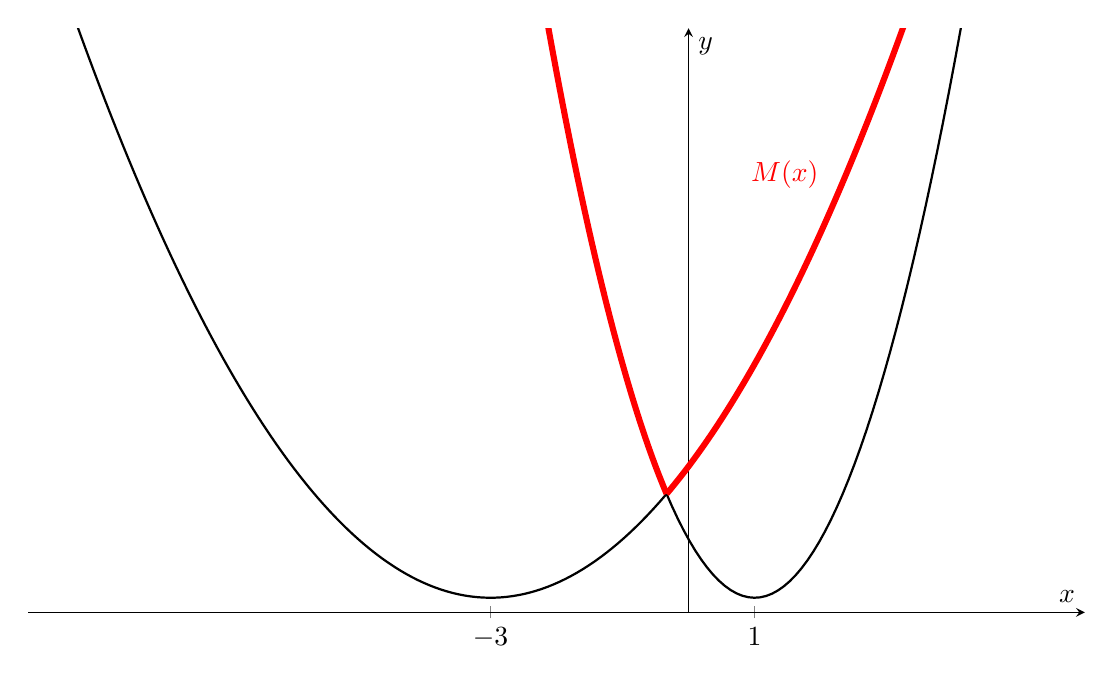
\begin{tikzpicture}
\begin{axis}[
    width=15cm, height=9cm,
    xmin=-10, xmax=6,
    ymin=0, ymax=40,
    axis lines=middle,
    xlabel={$x$}, ylabel={$y$},
    xtick={-3,1}, ytick=\empty,
    clip=true,
]
\addplot[black, line width=0.8pt, domain=-10:6, samples=180] {(x+3)^2+1};
\addplot[black, line width=0.8pt, domain=-10:6, samples=180] {4*(x-1)^2+1};
\addplot[red, line width=2.2pt, domain=-10:-1/3, samples=180] {4*(x-1)^2+1};
\addplot[red, line width=2.2pt, domain=-1/3:5, samples=140] {(x+3)^2+1};
\addplot[red, line width=2.2pt, domain=5:6, samples=35] {4*(x-1)^2+1};
\node[red,anchor=west] at (axis cs:0.8,30) {$M(x)$};
\end{axis}
\end{tikzpicture}
% end q000576 figure F2
\end{djsSolutionFigure}

From the graph, $M(x)$ is least at the intersection shown. We now find its exact position.

At an intersection, the two expressions are equal:
\[
(x+3)^2+1=4(x-1)^2+1
\]

Cancelling $1$ gives
\[
(x+3)^2=4(x-1)^2
\]

Expanding,
\[
x^2+6x+9=4x^2-8x+4
\]

Rearranging,
\[
3x^2-14x-5=0
\]

Factorising,
\[
(3x+1)(x-5)=0
\]

Hence the intersections occur at
\[
x=-\frac13\quad\text{or}\quad x=5
\]

The intersection shown is the one at $x=-\dfrac13$. 

Thus $M(x)$ is least when $x=-\dfrac13$, so the correct option is \textbf{C}.
% end q000576 solution
\end{djsSolution}
\end{enumerate}
\clearpage
\thispagestyle{djssolutions}
\vspace*{8pt}
\djsTopicLine{Number}
\begin{enumerate}[label=\textbf{\arabic*.},leftmargin=*,itemsep=0pt,start=15]
\questionitem[Number]
% begin q000583 stem
Let $N=2^6\times3^4\times5^3$

A positive factor $d$ of $N$ is chosen such that the highest common factor of $d$ and $\frac{N}{d}$ is $60$.

How many possible values of $d$ are there?
% end q000583 stem

\par\vspace*{12pt}
\begin{tabularx}{\linewidth}{@{}>{\bfseries}l Y@{}}
A &
% begin q000583 choice A
$2$
% end q000583 choice A
\\[0.8em]
B &
% begin q000583 choice B
$4$
% end q000583 choice B
\\[0.8em]
C &
% begin q000583 choice C
$6$
% end q000583 choice C
\\[0.8em]
D &
% begin q000583 choice D
$8$
% end q000583 choice D
\\[0.8em]
E &
% begin q000583 choice E
$12$
% end q000583 choice E
\\
\end{tabularx}

\begin{djsSolution}{D}
% begin q000583 solution
Write the factor as
\[
d=2^i3^j5^k
\]

where $0\leq i\leq6$, $0\leq j\leq4$ and $0\leq k\leq3$. The complementary factor is
\[
\frac Nd=2^{6-i}3^{4-j}5^{3-k}
\]

The highest common factor takes the smaller exponent of each prime in these two factors. Since
\[
60=2^2\times3\times5
\]
matching exponents gives
\[
\begin{aligned}
\min(i,6-i)&=2\\[6pt]
\min(j,4-j)&=1\\[6pt]
\min(k,3-k)&=1
\end{aligned}
\]

For the power of $2$, either $i=2$ or $6-i=2$. Both give the required minimum, so
\[
i=2\text{ or }i=4
\]

Similarly, the power of $3$ gives
\[
j=1\text{ or }j=3
\]
and the power of $5$ gives
\[
k=1\text{ or }k=2
\]

Each exponent therefore has two choices, and the choices are independent. The number of possible factors is
\[
2\times2\times2=8
\]

The correct option is \textbf{D}.
% end q000583 solution
\end{djsSolution}
\end{enumerate}
\clearpage
\thispagestyle{djssolutions}
\vspace*{8pt}
\djsTopicLine{Polynomials}
\begin{enumerate}[label=\textbf{\arabic*.},leftmargin=*,itemsep=0pt,start=16]
\questionitem[Polynomials]
% begin q000072 stem
Consider
\[P(x)=x^4+ax^3+bx^2+ax+1\]
where $a$ and $b$ are real constants.

Suppose $(x-2)$ and $\left(x+\frac{1}{2}\right)$ are both factors of $P(x)$

What is the value of $b$?
% end q000072 stem

\par\vspace*{12pt}
\begin{tabularx}{\linewidth}{@{}>{\bfseries}l Y@{}}
A &
% begin q000072 choice A
$-13$
% end q000072 choice A
\\[0.8em]
B &
% begin q000072 choice B
$-5$
% end q000072 choice B
\\[0.8em]
C &
% begin q000072 choice C
$0$
% end q000072 choice C
\\[0.8em]
D &
% begin q000072 choice D
$5$
% end q000072 choice D
\\[0.8em]
E &
% begin q000072 choice E
$13$
% end q000072 choice E
\\[0.8em]
F &
% begin q000072 choice F
$-\frac{17}{4}$
% end q000072 choice F
\\
\end{tabularx}

\begin{djsSolution}{F}
% begin q000072 solution
By the factor theorem, if $(x-r)$ is a factor of $P(x)$, then $P(r)=0$.

The two given factors therefore give $P(2)=0$ and $P\left(-\frac12\right)=0$.

Substituting $x=2$ gives
\[
16+8a+4b+2a+1=0
\]

Collecting terms,
\[
17+10a+4b=0
\]

Now substitute $x=-\frac12$:
\[
\begin{aligned}
P\left(-\frac12\right)
&=\frac1{16}-\frac a8+\frac b4-\frac a2+1\\[8pt]
&=\frac{17}{16}-\frac a8+\frac b4-\frac a2\\[8pt]
&=\frac{17}{16}-\frac{5a}{8}+\frac b4
\end{aligned}
\]

Since this is zero, multiplying by $16$ gives
\[
17-10a+4b=0
\]

Adding the two equations eliminates $a$:
\[
34+8b=0
\]

Rearranging,
\[
8b=-34
\]

Hence
\[
b=-\frac{17}{4}
\]

The correct option is \textbf{F}.
% end q000072 solution
\end{djsSolution}
\end{enumerate}
\clearpage
\thispagestyle{djssolutions}
\vspace*{8pt}
\djsTopicLine{Integration}
\begin{enumerate}[label=\textbf{\arabic*.},leftmargin=*,itemsep=0pt,start=17]
\questionitem[Integration]
% begin q000614 stem
Let $k$ be a positive constant. The curve $C$ has equation \[y = x^3 - 3k^2 x + 2k^3\]
The point $A$ is the local maximum of $C$.

The line parallel to the $x$-axis passing through $A$ intersects $C$ again at the point $B$.

The area of the region bounded by $C$ and the line segment $AB$ is $108$.

What is the value of $k$?
% end q000614 stem

\par\vspace*{12pt}
\begin{tabularx}{\linewidth}{@{}>{\bfseries}l Y@{}}
A &
% begin q000614 choice A
$1$
% end q000614 choice A
\\[0.8em]
B &
% begin q000614 choice B
$\sqrt{2}$
% end q000614 choice B
\\[0.8em]
C &
% begin q000614 choice C
$\sqrt{3}$
% end q000614 choice C
\\[0.8em]
D &
% begin q000614 choice D
$2$
% end q000614 choice D
\\[0.8em]
E &
% begin q000614 choice E
$2\sqrt{2}$
% end q000614 choice E
\\[0.8em]
F &
% begin q000614 choice F
$3$
% end q000614 choice F
\\[0.8em]
G &
% begin q000614 choice G
$4$
% end q000614 choice G
\\
\end{tabularx}

\begin{djsSolution}{D}
% begin q000614 solution
Differentiate to find the stationary points:
\[
\frac{\mathrm{d}y}{\mathrm{d}x}=3x^2-3k^2
\]

Factorising gives
\[
\frac{\mathrm{d}y}{\mathrm{d}x}=3(x-k)(x+k)
\]

Hence
\[
x=-k\quad\text{or}\quad x=k
\]

Substituting $x=-k$ into the equation of $C$ gives
\[
y=(-k)^3-3k^2(-k)+2k^3=4k^3
\]

Substituting $x=k$ gives
\[
y=k^3-3k^2(k)+2k^3=0
\]

Since $k>0$, the gradient changes from positive to negative at $x=-k$, then from negative to positive at $x=k$. 

Thus $A$ is $(-k,4k^3)$ and the local minimum is $(k,0)$, giving this sketch of $C$:

\begin{djsSolutionFigure}
% begin q000614 figure F1
\begin{tikzpicture}[x=2.5cm,y=0.85cm]
\coordinate (A) at (-1,4);
\coordinate (M) at (1,0);
\draw[->,thick,black] (-2.4,0) -- (2.42,0) node[right] {$x$};
\draw[->,thick,black] (0,-3.1) -- (0,7.1) node[above] {$y$};
\draw[thick,black] plot[domain=-2.25:2.22,samples=180,variable=\t] (\t,{\t*\t*\t-3*\t+2});
\node[above left=4pt] at (A) {$A(-k,4k^3)$};
\node[below right=4pt] at (M) {$(k,0)$};
\node[above left] at (-1.8,{-1.8*1.8*1.8+3*1.8+2}) {$C$};
\end{tikzpicture}
% end q000614 figure F1
\end{djsSolutionFigure}

The line through $A$ parallel to the $x$-axis is
\[
y=4k^3
\]

To find its other intersection with $C$, set the two expressions for $y$ equal:
\[
x^3-3k^2x+2k^3=4k^3
\]

Rearranging gives
\[
x^3-3k^2x-2k^3=0
\]

The line touches $C$ at the stationary point $A$, so $x=-k$ is a double root of this equation. Factorising gives
\[
(x+k)^2(x-2k)=0
\]

The other intersection therefore has $x=2k$, so
\[
B=(2k,4k^3)
\]

Adding $AB$ to the sketch shows the bounded region:

\begin{djsSolutionFigure}
% begin q000614 figure F2
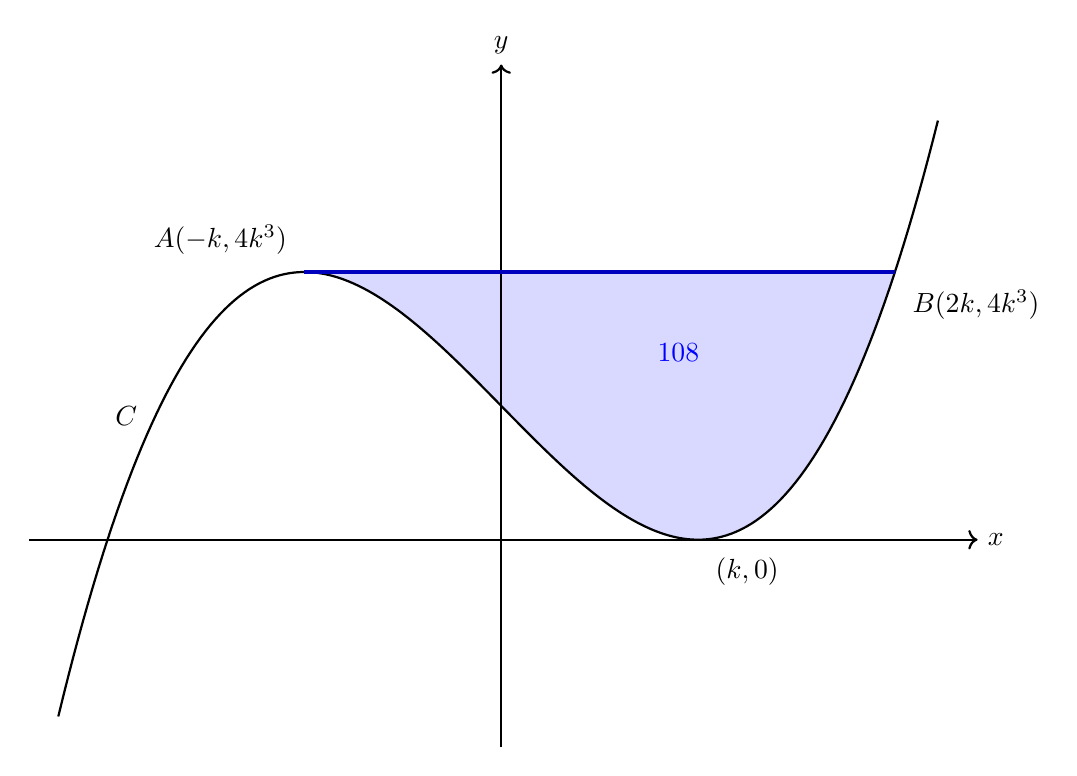
\begin{tikzpicture}[x=2.5cm,y=0.85cm]
\coordinate (A) at (-1,4);
\coordinate (M) at (1,0);
\coordinate (B) at (2,4);
\path[fill=blue!15] (A) -- (B) -- plot[domain=2:-1,samples=120,variable=\t] (\t,{\t*\t*\t-3*\t+2}) -- cycle;
\draw[->,thick,black] (-2.4,0) -- (2.42,0) node[right] {$x$};
\draw[->,thick,black] (0,-3.1) -- (0,7.1) node[above] {$y$};
\draw[thick,black] plot[domain=-2.25:2.22,samples=180,variable=\t] (\t,{\t*\t*\t-3*\t+2});
\draw[blue!75!black,line width=1.3pt] (A) -- (B);
\node[above left=4pt] at (A) {$A(-k,4k^3)$};
\node[below right=4pt] at (M) {$(k,0)$};
\node[above left] at (-1.8,{-1.8*1.8*1.8+3*1.8+2}) {$C$};
\node[below right=4pt] at (B) {$B(2k,4k^3)$};
\node[blue] at (0.9,2.8) {$108$};
\end{tikzpicture}
% end q000614 figure F2
\end{djsSolutionFigure}

Between $x=-k$ and $x=2k$, the line is above the curve: their difference is $(x+k)^2(2k-x)$, which is non-negative there. 

For an upper graph $f(x)$ and a lower graph $g(x)$, the formula for the area between the graphs is
\[
\text{Area}=\int_a^b\bigl(f(x)-g(x)\bigr)\,\mathrm{d}x
\]

Here $f(x)=4k^3$ and $g(x)=x^3-3k^2x+2k^3$. Using the given area,
\[
108=\int_{-k}^{2k}\bigl(4k^3-(x^3-3k^2x+2k^3)\bigr)\,\mathrm{d}x
\]

Simplifying the integrand gives
\[
108=\int_{-k}^{2k}(-x^3+3k^2x+2k^3)\,\mathrm{d}x
\]

Integrating gives
\[
108=\left[-\frac{x^4}{4}+\frac{3k^2x^2}{2}+2k^3x\right]_{-k}^{2k}
\]

Substituting the limits gives
\[
108=\left(-\frac{(2k)^4}{4}+\frac{3k^2(2k)^2}{2}+2k^3(2k)\right)-\left(-\frac{(-k)^4}{4}+\frac{3k^2(-k)^2}{2}+2k^3(-k)\right)
\]

Simplifying gives
\[
108=6k^4-\left(-\frac{3k^4}{4}\right)
\]

Therefore
\[
108=\frac{27k^4}{4}
\]

Rearranging gives
\[
k^4=16
\]

Since $k$ is positive,
\[
k=2
\]
The correct option is \textbf{D}.
% end q000614 solution
\end{djsSolution}
\end{enumerate}
\clearpage
\thispagestyle{djssolutions}
\vspace*{8pt}
\djsTopicLine{Algebra}
\begin{enumerate}[label=\textbf{\arabic*.},leftmargin=*,itemsep=0pt,start=18]
\questionitem[Algebra]
% begin q000135 stem
Let $a$ and $b$ be real numbers with $a+b=1$

What is the least possible value of \[(a^2 + b)(b^2 + a)\quad?\]
% end q000135 stem

\par\vspace*{12pt}
\begin{tabularx}{\linewidth}{@{}>{\bfseries}l Y@{}}
A &
% begin q000135 choice A
$\dfrac{9}{16}$
% end q000135 choice A
\\[0.8em]
B &
% begin q000135 choice B
$\dfrac{1}{4}$
% end q000135 choice B
\\[0.8em]
C &
% begin q000135 choice C
$\dfrac{1}{2}$
% end q000135 choice C
\\[0.8em]
D &
% begin q000135 choice D
$\dfrac{3}{4}$
% end q000135 choice D
\\[0.8em]
E &
% begin q000135 choice E
$1$
% end q000135 choice E
\\
\end{tabularx}

\begin{djsSolution}{A}
% begin q000135 solution
Using $b=1-a$, substitute into the product:
\[
(a^2+b)(b^2+a)=\bigl(a^2+1-a\bigr)\bigl((1-a)^2+a\bigr)
\]
Expanding the second factor gives
\[
(1-a)^2+a=1-2a+a^2+a=a^2-a+1
\]
The two factors are therefore equal, so
\[
(a^2+b)(b^2+a)=(a^2-a+1)^2
\]
Complete the square inside the brackets:
\[
\begin{aligned}
a^2-a+1
&=\left(a-\frac12\right)^2-\frac14+1\\[8pt]
&=\left(a-\frac12\right)^2+\frac34
\end{aligned}
\]
The squared term is at least $0$, with equality when $a=\frac12$. Thus the expression inside the outer square has minimum $\frac34$, which is positive. 

Squaring a positive number increases as that number increases, so the product has minimum
\[
\left(\frac34\right)^2=\frac{9}{16}
\]
This is attained when $a=\frac12$ and $b=\frac12$. The correct option is \textbf{A}.
% end q000135 solution
\end{djsSolution}
\end{enumerate}
\clearpage
\thispagestyle{djssolutions}
\vspace*{8pt}
\djsTopicLine{Functions \& Graphs}
\begin{enumerate}[label=\textbf{\arabic*.},leftmargin=*,itemsep=0pt,start=19]
\questionitem[Functions \& Graphs]
% begin q000626 stem
The diagram shows the graph of $y=f(x)$, where $f(x)=x^3-3x$. The horizontal lines through the turning points are also shown. \\

How many distinct real solutions does the equation $f(f(x))=f(x)$ have?
% end q000626 stem

\begin{center}
% begin q000626 diagram
\begin{tikzpicture}
\pgfmathsetmacro{\curveLabelX}{-2.08}
\pgfmathsetmacro{\curveLabelY}{\curveLabelX^3-3*\curveLabelX}

\begin{axis}[
    width=8cm,
    height=10cm,
    axis equal image,
    axis lines=middle,
    axis line style={black,-{Stealth[length=2.5mm]}},
    xlabel={$x$},
    ylabel={$y$},
    xlabel style={at={(axis description cs:1,0.5)},anchor=west},
    ylabel style={at={(axis description cs:0.5,1)},anchor=south},
    xmin=-2.3,
    xmax=2.3,
    ymin=-3,
    ymax=3,
    xtick={-2,-1,1,2},
    ytick={0},
    tick align=outside,
    grid=none,
    clip=true,
]

\addplot[dashed, black, domain=-2.3:2.3, samples=2] {2};
\addplot[dashed, black, domain=-2.3:2.3, samples=2] {-2};

\addplot[thick, black, domain=-2.3:2.3, samples=180]
    {x^3-3*x};

\node[below left] at (axis cs:0,0) {$O$};
\node[right] at (axis cs:\curveLabelX,\curveLabelY) {$y=f(x)$};

\coordinate (Ytwo) at (axis cs:2.3,2);
\coordinate (YminusTwo) at (axis cs:2.3,-2);

\end{axis}

\node[right] at (Ytwo) {$y=2$};
\node[right] at (YminusTwo) {$y=-2$};

\end{tikzpicture}
% end q000626 diagram
\end{center}

\par\vspace*{12pt}
\begin{tabularx}{\linewidth}{@{}>{\bfseries}l Y@{}}
A &
% begin q000626 choice A
$5$
% end q000626 choice A
\\[0.8em]
B &
% begin q000626 choice B
$6$
% end q000626 choice B
\\[0.8em]
C &
% begin q000626 choice C
$7$
% end q000626 choice C
\\[0.8em]
D &
% begin q000626 choice D
$8$
% end q000626 choice D
\\[0.8em]
E &
% begin q000626 choice E
$9$
% end q000626 choice E
\\
\end{tabularx}

\begin{djsSolution}{C}
% begin q000626 solution
Put $u=f(x)$. Then the equation becomes $f(u)=u$: we first need to find which outputs of $f$ are equal to their own input.

On the graph, $f(u)=u$ holds where $y=f(x)$ meets $y=x$. Adding that line shows crossings at $(-2,-2)$, $(0,0)$ and $(2,2)$.

To confirm that these are all the possible values of $u$, factor the equation:
\[
u^3-3u=u
\]
Rearranging,
\[
u^3-4u=0
\]
Factorising,
\[
u(u-2)(u+2)=0
\]
Hence
\[
u=-2\text{ or }u=0\text{ or }u=2
\]

\begin{djsSolutionFigure}
% begin q000626 figure F1
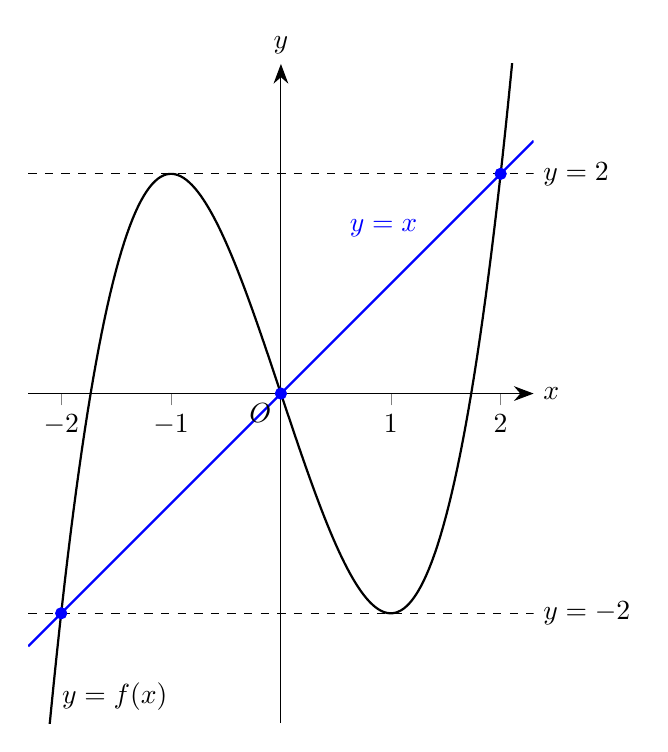
\begin{tikzpicture}
\pgfmathsetmacro{\curveLabelX}{-2.08}
\pgfmathsetmacro{\curveLabelY}{\curveLabelX^3-3*\curveLabelX}

\begin{axis}[
    width=8cm,
    height=10cm,
    axis equal image,
    axis lines=middle,
    axis line style={black,-{Stealth[length=2.5mm]}},
    xlabel={$x$},
    ylabel={$y$},
    xlabel style={at={(axis description cs:1,0.5)},anchor=west},
    ylabel style={at={(axis description cs:0.5,1)},anchor=south},
    xmin=-2.3,
    xmax=2.3,
    ymin=-3,
    ymax=3,
    xtick={-2,-1,1,2},
    ytick={0},
    tick align=outside,
    grid=none,
    clip=true,
]

\addplot[dashed, black, domain=-2.3:2.3, samples=2] {2};
\addplot[dashed, black, domain=-2.3:2.3, samples=2] {-2};

\addplot[thick, black, domain=-2.3:2.3, samples=180]
    {x^3-3*x};

\addplot[thick, blue, domain=-2.3:2.3, samples=2] {x}
    node[pos=0.79, above left, blue] {$y=x$};
\addplot[only marks, mark=*, mark size=2pt, blue]
    coordinates {(-2,-2) (0,0) (2,2)};

\node[below left] at (axis cs:0,0) {$O$};
\node[right] at (axis cs:\curveLabelX,\curveLabelY) {$y=f(x)$};

\coordinate (Ytwo) at (axis cs:2.3,2);
\coordinate (YminusTwo) at (axis cs:2.3,-2);

\end{axis}

\node[right] at (Ytwo) {$y=2$};
\node[right] at (YminusTwo) {$y=-2$};

\end{tikzpicture}
% end q000626 figure F1
\end{djsSolutionFigure}


Now count the inputs $x$ that produce each of these three outputs. 

For each value of $u$, draw the horizontal line $y=u$; its intersections with the curve are the solutions of $f(x)=u$. 

The lines $y=-2$ and $y=2$ are already on the given graph, while $y=0$ is the $x$-axis.

\begin{djsSolutionFigure}
% begin q000626 figure F2
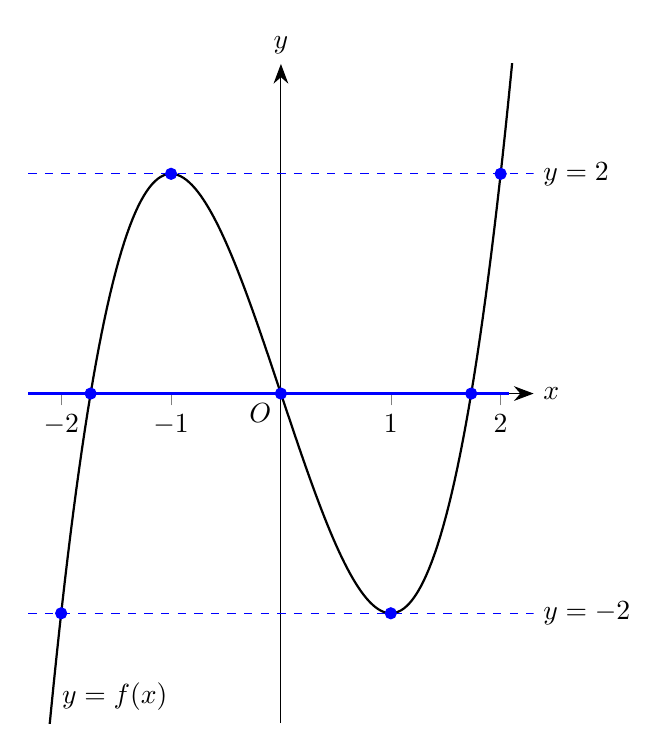
\begin{tikzpicture}
\pgfmathsetmacro{\curveLabelX}{-2.08}
\pgfmathsetmacro{\curveLabelY}{\curveLabelX^3-3*\curveLabelX}
\pgfmathsetmacro{\leftRoot}{-sqrt(3)}
\pgfmathsetmacro{\rightRoot}{sqrt(3)}

\begin{axis}[
    width=8cm,
    height=10cm,
    axis equal image,
    axis lines=middle,
    axis line style={black,-{Stealth[length=2.5mm]}},
    xlabel={$x$},
    ylabel={$y$},
    xlabel style={at={(axis description cs:1,0.5)},anchor=west},
    ylabel style={at={(axis description cs:0.5,1)},anchor=south},
    xmin=-2.3,
    xmax=2.3,
    ymin=-3,
    ymax=3,
    xtick={-2,-1,1,2},
    ytick={0},
    tick align=outside,
    grid=none,
    clip=true,
]

\addplot[dashed, blue, domain=-2.3:2.3, samples=2] {2};
\addplot[dashed, blue, domain=-2.3:2.3, samples=2] {-2};
\draw[blue, line width=1.1pt] (axis cs:-2.3,0) -- (axis cs:2.08,0);

\addplot[thick, black, domain=-2.3:2.3, samples=180]
    {x^3-3*x};

\addplot[only marks, mark=*, mark size=2pt, blue]
    coordinates {(-2,-2) (1,-2) (\leftRoot,0) (0,0)
                 (\rightRoot,0) (-1,2) (2,2)};

\node[below left] at (axis cs:0,0) {$O$};
\node[right] at (axis cs:\curveLabelX,\curveLabelY) {$y=f(x)$};

\coordinate (Ytwo) at (axis cs:2.3,2);
\coordinate (YminusTwo) at (axis cs:2.3,-2);

\end{axis}

\node[right] at (Ytwo) {$y=2$};
\node[right] at (YminusTwo) {$y=-2$};

\end{tikzpicture}
% end q000626 figure F2
\end{djsSolutionFigure}

The line $y=-2$ crosses the curve at $x=-2$ and touches it at $x=1$. It therefore gives
\[
u=-2:\quad 2\text{ distinct solutions}
\]

The line $y=0$ crosses the curve three times: once on each side of the origin and once at the origin. It gives
\[
u=0:\quad 3\text{ distinct solutions}
\]

The line $y=2$ touches the curve at $x=-1$ and crosses it at $x=2$. It gives
\[
u=2:\quad 2\text{ distinct solutions}
\]

No input $x$ can produce two different values of $u$, so these counts do not overlap. The total is
\[
2+3+2=7
\]

The correct option is \textbf{C}.

The substitution $u=f(x)$ is useful because $f(x)$ is both the input of the outer $f$ and the whole right-hand side. Solving $f(u)=u$ identifies the possible outputs first; the horizontal lines then count the inputs producing each output. 
% end q000626 solution
\end{djsSolution}
\end{enumerate}
\clearpage
\thispagestyle{djssolutions}
\vspace*{8pt}
\djsTopicLine{Inequalities}
\begin{enumerate}[label=\textbf{\arabic*.},leftmargin=*,itemsep=0pt,start=20]
\questionitem[Inequalities]
% begin q000154 stem
Let $f(x)=ax^2+bx+c$ be a quadratic function with real coefficients such that $f(x)\ge 0$ for all real $x$

Suppose that for every real $x$, \[ f(x+1)-f(x)\ge 2x+3 \] What is the smallest possible value of $f(0)$?
% end q000154 stem

\par\vspace*{12pt}
\begin{tabularx}{\linewidth}{@{}>{\bfseries}l Y@{}}
A &
% begin q000154 choice A
$0$
% end q000154 choice A
\\[0.8em]
B &
% begin q000154 choice B
$\dfrac{1}{4}$
% end q000154 choice B
\\[0.8em]
C &
% begin q000154 choice C
$1$
% end q000154 choice C
\\[0.8em]
D &
% begin q000154 choice D
$2$
% end q000154 choice D
\\[0.8em]
E &
% begin q000154 choice E
$\dfrac{9}{4}$
% end q000154 choice E
\\[0.8em]
F &
% begin q000154 choice F
$4$
% end q000154 choice F
\\[0.8em]
G &
% begin q000154 choice G
$\dfrac{25}{4}$
% end q000154 choice G
\\
\end{tabularx}

\begin{djsSolution}{C}
% begin q000154 solution
Since $f$ is a quadratic that is non-negative for every real $x$, it opens upwards, so $a>0$. Its discriminant must satisfy
\[
b^2-4ac\leq0
\]

Now expand the difference in the given inequality:
\[
\begin{aligned}
f(x+1)-f(x)
&=a(x+1)^2+b(x+1)+c-(ax^2+bx+c)\\
&=2ax+a+b
\end{aligned}
\]

Thus the inequality becomes
\[
2ax+a+b\geq2x+3
\]

Rearranging,
\[
2(a-1)x+(a+b-3)\geq0
\]

This must hold for every real $x$. The left-hand side is a linear expression, whose graph is a straight line. Any straight line with a non-zero gradient goes below the horizontal axis in one direction:
\begin{itemize}
\item If $a>1$, the gradient is positive, so sufficiently large negative values of $x$ make the expression negative.
\item If $a<1$, the gradient is negative, so sufficiently large positive values of $x$ make the expression negative.
\end{itemize}

Both possibilities contradict the inequality. The line must therefore be horizontal, so its gradient is zero:
\[
2(a-1)=0
\]

Hence
\[
a=1
\]

Substituting this into the inequality leaves
\[
b-2\geq0
\]
so
\[
b\geq2
\]

The discriminant condition for $f$ now becomes
\[
b^2-4c\leq0
\]

Rearranging and using $b\geq2$,
\[
c\geq\frac{b^2}{4}\geq1
\]

To check that this lower bound can be achieved, take $a=1$, $b=2$ and $c=1$. Then
\[
f(x)=(x+1)^2\geq0
\]
for every real $x$, and
\[
f(x+1)-f(x)=(x+2)^2-(x+1)^2=2x+3
\]

Thus both conditions are satisfied, and the smallest possible value of $f(0)=c$ is
\[
f(0)=1
\]

The correct option is \textbf{C}.
% end q000154 solution
\end{djsSolution}
\end{enumerate}
\end{document}
